%% ----------------------------------------------------------------
%% Project Report.tex
%% ---------------------------------------------------------------- 
\documentclass[sotoncolour]{uosprogress}    % Use the progress Style with custom link colour
\graphicspath{{./Figures/}}   % Location of your graphics files
\usepackage{xurl}
\usepackage{amsmath, mathtools}
\usepackage[square, numbers]{natbib}            % Use Natbib style for the refs.
\usepackage[final]{pdfpages}
\usepackage{lscape}
\hypersetup{colorlinks=true}   % Set to false for black/white printing
%% ----------------------------------------------------------------
%% Definitions.tex
%% ---------------------------------------------------------------- 
\newcommand{\BibTeX}{{\rm B\kern-.05em{\sc i\kern-.025em b}\kern-.08em T\kern-.1667em\lower.7ex\hbox{E}\kern-.125emX}}

%% People
\newcounter{address}
\setcounter{address}{1}
\renewcommand{\theaddress}{\textsuperscript{\fnsymbol{address}}}
\newcommand{\address}[1]{\refstepcounter{address}\theaddress#1\\}
\newcommand{\Name}[3]{\texorpdfstring{\href{mailto:#3}{#2}#1}{#2}\xspace}
\newcommand{\SteveRGunn}[1]{\Name{#1}{Steve R. Gunn}{S.R.Gunn@ecs.soton.ac.uk}}

%% Dingbats
\newcommand{\tick}{\ding{51}}
\newcommand{\cross}{\ding{55}}

%% Calculus
\newcommand{\pd}[2]{\ensuremath{\frac{\partial #1}{\partial #2}}\xspace}
\newcommand{\fd}[2]{\ensuremath{\frac{d #1}{d #2}}\xspace}
\newcommand{\dint}{\ensuremath{\int\!\!\!\int}\xspace}
\newcommand{\tint}{\ensuremath{\int\!\!\!\int\!\!\!\int}\xspace}

%% Math Sets
\newcommand{\Q}[1]{\ensuremath{\mathbb{#1}}\xspace}
\newcommand{\R}{\Q{R}}

%% Matrix, Vector
\newcommand{\V}[1]{\ensuremath{\boldsymbol{#1}}\xspace}
\newcommand{\M}[1]{\ensuremath{\boldsymbol{#1}}\xspace}
\newcommand{\0}{\V{0}}
\newcommand{\1}{\V{1}}
\newcommand{\I}{\M{I}}

%% Math Functions
\newcommand{\F}[1]{\ensuremath{\mathrm{#1}}\xspace}
\newcommand{\sgn}{\F{sgn}}
\newcommand{\tr}{\F{trace}}
\newcommand{\diag}{\F{diag}}

%% Math Names
\newcommand{\N}[1]{\ensuremath{\mathit{#1}}\xspace}

%% Data
\newcommand{\mc}[1]{\ensuremath{\mathcal{#1}}\xspace}
\newcommand{\Hyp}{\mc{H}}
\newcommand{\D}{\mc{D}}

%% Kernel
\newcommand{\K}{\M{K}}
\newcommand{\eins}{\texorpdfstring{\ensuremath{\epsilon}}{\textepsilon}-insensitive\xspace}
\newcommand{\e}{\ensuremath{\epsilon}\xspace}
\newcommand{\Bxi}{\ensuremath{\boldsymbol{\xi}}\xspace}
\newcommand{\Kanova}{\ensuremath{\mathit{K_{ANOVA}}}\xspace}
\newcommand{\Kspline}{\ensuremath{\mathit{K_{spline}}}\xspace}

%% Bayesian
\newcommand{\MP}{\ensuremath{\mathit{{\scriptscriptstyle \hspace{-1.5pt}M\hspace{-1.5pt}P}}}\xspace}
\newcommand{\ML}{\ensuremath{\mathit{{\scriptscriptstyle \hspace{-1.5pt}M\hspace{-1.5pt}L}}}\xspace}
\newcommand{\Qw}{\ensuremath{Q_{\w}(\w)}\xspace}
\newcommand{\Qa}{\ensuremath{Q_{\Ba}(\Ba)}\xspace}
\newcommand{\Qb}{\ensuremath{Q_{\beta}(\beta)}\xspace}
\newcommand{\wMPab}{\ensuremath{\w_{\MP|\bar {\Ba},\bar \beta}}\xspace}
\newcommand{\wMP}{\ensuremath{\w_{\MP}}\xspace}
\newcommand{\yMP}{\ensuremath{y_{\MP}}\xspace}
\newcommand{\BaMP}{\ensuremath{\Ba_{\hspace{1pt}\MP}}\xspace}
\newcommand{\aMP}{\ensuremath{\alpha_{\hspace{1pt}\MP}}\xspace}
\newcommand{\bMP}{\ensuremath{\beta_{\hspace{1pt}\MP}}\xspace}
\newcommand{\Sab}{\ensuremath{\M{\Sigma}_{\bar \Ba,\bar \beta}}\xspace}
\newcommand{\Ba}{\ensuremath{\boldsymbol{\alpha}}\xspace}
\newcommand{\Bb}{\ensuremath{\boldsymbol{\beta}}\xspace}
\newcommand{\Bm}{\ensuremath{\boldsymbol{\mu}}\xspace}
\newcommand{\BL}{\ensuremath{\boldsymbol{\Lambda}}\xspace}
\newcommand{\BPhi}{\ensuremath{\boldsymbol{\Phi}}\xspace}
\newcommand{\SMP}{\ensuremath{\M{\Sigma}_{\MP}}\xspace}

\newcommand{\Pa}{\ensuremath{P(\alpha|\mathcal{H})}\xspace}
\newcommand{\Pb}{\ensuremath{P(\beta|\mathcal{H})}\xspace}
\newcommand{\Pab}{\ensuremath{P(\alpha,\beta|\mathcal{H})}\xspace}
\newcommand{\Pw}{\ensuremath{P(\w|\mathcal{H})}\xspace}
\newcommand{\PD}{\ensuremath{P(\D|\mathcal{H})}\xspace}
\newcommand{\PwIa}{\ensuremath{P(\w|\alpha,\mathcal{H})}\xspace}
\newcommand{\PDIwb}{\ensuremath{P(\D|\w,\beta,\mathcal{H})}\xspace}
\newcommand{\PDwab}{\ensuremath{P(\D,\w,\alpha,\beta|\mathcal{H})}\xspace}
\newcommand{\PDIw}{\ensuremath{P(\D|\w,\mathcal{H})}\xspace}
\newcommand{\PwID}{\ensuremath{P(\w|\D,\mathcal{H})}\xspace}
\newcommand{\PwabID}{\ensuremath{P(\w,\alpha,\beta|\D,\mathcal{H})}\xspace}

\newcommand{\PanH}{\ensuremath{P(\alpha)}\xspace}
\newcommand{\PbnH}{\ensuremath{P(\beta)}\xspace}
\newcommand{\PabnH}{\ensuremath{P(\alpha,\beta)}\xspace}
\newcommand{\PwnH}{\ensuremath{P(\w)}\xspace}
\newcommand{\PDnH}{\ensuremath{P(\D)}\xspace}
\newcommand{\PwIanH}{\ensuremath{P(\w|\alpha)}\xspace}
\newcommand{\PDIwbnH}{\ensuremath{P(\D|\w,\beta)}\xspace}
\newcommand{\PDwabnH}{\ensuremath{P(\D,\w,\Ba,\beta)}\xspace}
\newcommand{\PDIwnH}{\ensuremath{P(\D|\w)}\xspace}
\newcommand{\PwIDnH}{\ensuremath{P(\w|\D)}\xspace}
\newcommand{\PwabIDnH}{\ensuremath{P(\w,\alpha,\beta|\D)}\xspace}

\newcommand{\PDwBab}{\ensuremath{P(\D,\w,\Ba,\beta|\mathcal{H})}\xspace}
\newcommand{\PwIBa}{\ensuremath{P(\w|\Ba,\mathcal{H})}\xspace}
\newcommand{\PBab}{\ensuremath{P(\Ba,\beta|\mathcal{H})}\xspace}
\newcommand{\PwBabID}{\ensuremath{P(\w,\Ba,\beta|\D,\mathcal{H})}\xspace}

\newcommand{\PBanH}{\ensuremath{P(\Ba)}\xspace}
\newcommand{\PwIBanH}{\ensuremath{P(\w|\Ba)}\xspace}

%% Snakes
\newcommand{\Esnake}{\ensuremath{\mathit{E_{snake}}}\xspace}
\newcommand{\Eimage}{\ensuremath{\mathit{E_{image}}}\xspace}
\newcommand{\Econt}{\ensuremath{\mathit{E_{cont}}}\xspace}
\newcommand{\Ecurv}{\ensuremath{\mathit{E_{curv}}}\xspace}
\newcommand{\Eint}{\ensuremath{\mathit{E_{int}}}\xspace}
\newcommand{\Eext}{\ensuremath{\mathit{E_{ext}}}\xspace}
\newcommand{\Eterm}{\ensuremath{\mathit{E_{term}}}\xspace}
\newcommand{\Eline}{\ensuremath{\mathit{E_{line}}}\xspace}
\newcommand{\Eedge}{\ensuremath{\mathit{E_{edge}}}\xspace}
\newcommand{\Econ}{\ensuremath{\mathit{E_{con}}}\xspace}
\newcommand{\Eangle}{\ensuremath{\mathit{E_{angle}}}\xspace}
\newcommand{\Elshape}{\ensuremath{\mathit{E_{lshape}}}\xspace}
\newcommand{\Eedgedir}{\ensuremath{\mathit{E_{edgedir}}}\xspace}
\newcommand{\Emodel}{\ensuremath{\mathit{E_{model}}}\xspace}
\newcommand{\wte}{\ensuremath{\mathit{w_{term}}}\xspace}
\newcommand{\wli}{\ensuremath{\mathit{w_{line}}}\xspace}
\newcommand{\wed}{\ensuremath{\mathit{w_{edge}}}\xspace}
\newcommand{\wco}{\ensuremath{\mathit{w_{con}}}\xspace}

%% Environments
\newcounter{alg}
\newenvironment{algorithm}[1]
{
    \stepcounter{alg}
    \begin{table}[htb]
    \centering
    \begin{tabular}[t]{ll}
    \hline&\\
    \multicolumn{2}{l}{\bf Algorithm \arabic{alg}: #1}\\&\\
} {
    &\\
    \hline
    \end{tabular}
    \end{table}
}
            % Include your abbreviations
%% ----------------------------------------------------------------
%% --------------------THESIS/DOC INFORMATION ---------------------
\faculty     {Faculty of Physical Sciences and Engineering}
\FACULTY     {\MakeUppercase{\facname}}
\department  {Electronics and Computer Science}
\DEPARTMENT  {\MakeUppercase{\deptname}}
\group       {}
\GROUP       {\MakeUppercase{\groupname}}
\title      {A Deep Learning Method for Traffic Prediction}
\authors    {\texorpdfstring
            {\href{mailto:yz25g21@soton.ac.uk}{Yanzhe S. Zhang}}
            {}
            }
\addresses  {\groupname\\\deptname\\\univname}
\date       {\today}
\supervisor {Professor Lie-Liang Yang}
\examiner   {Mr. Iain McNally}
%% Optional Fields TODO: Replace these fields with your own data

\qualifications{MEng}
\subject    {Part III Individual Project}
\keywords   {}

\begin{document}

%% ------------------ FRONT MATTER ORGANISATION -------------------
\frontmatter
\maketitle

\begin{abstract}
    This is the project report of the Part III Project. 

    In contemporary urban environments, efficient urban mobility is imperative for daily routines. 
    Traffic congestion stands as a pervasive challenge in urban areas, leading to delays, frustration, and inefficiencies in transportation systems. 
    This project aims to explore traffic predictions based on historical data using deep learning techniques. 
    This provides insights into improving urban mobility and effectively managing traffic congestion.
    
    Various neural network architectures were developed and evaluated, with a comprehensive analysis of the influence of different hyper-parameters on performance. 
    Specifically, the project investigates two prediction approaches: localised predictions for specific locations within the urban map and global predictions covering the entire area. 
\end{abstract}

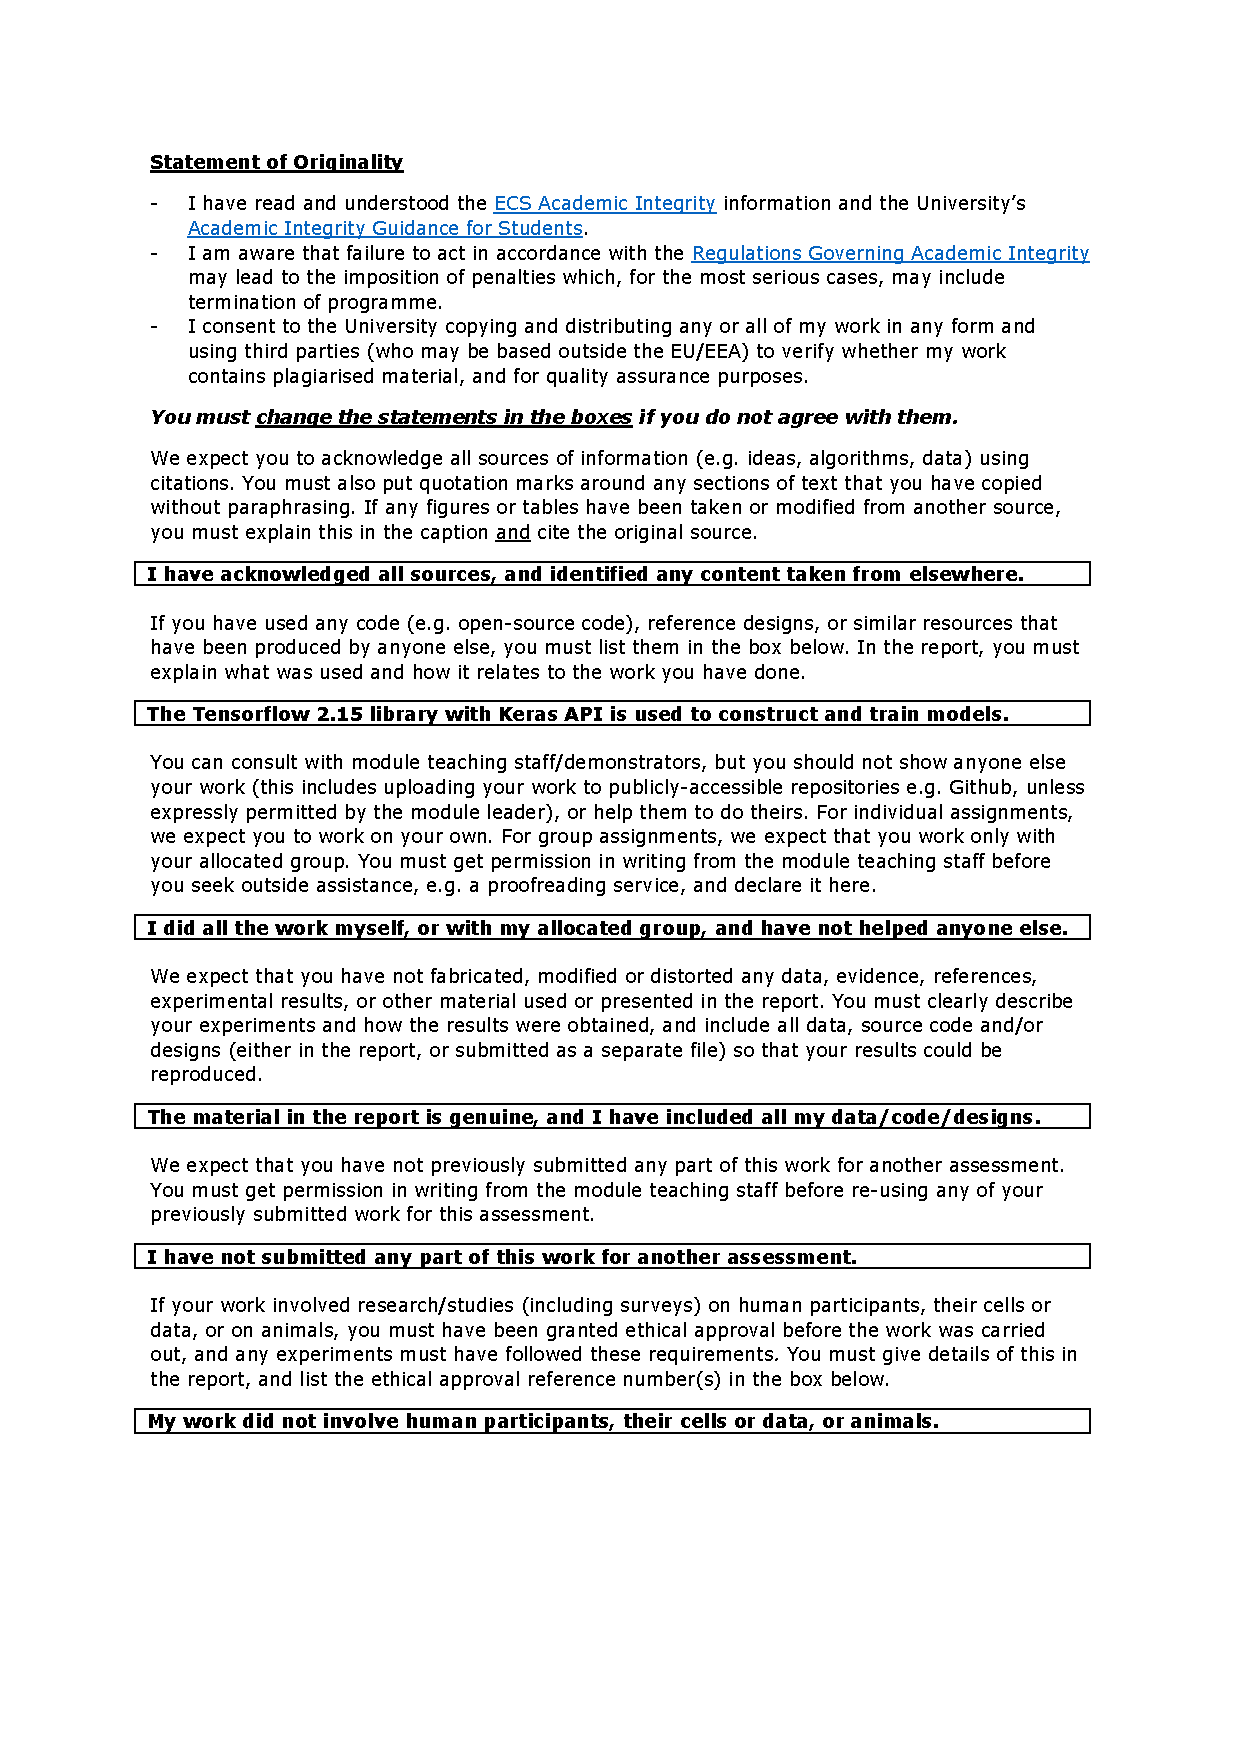
\includepdf{ai_statement.pdf}
% \acknowledgements

\let\cleardoublepage\clearpage

\pdfbookmark[0]{\contentsname}{toc} % Add pdf bookmark for contents page for navigation

\tableofcontents
% \listoffigures
% \listoftables

%% The List of listings does not, by default, appear in the ToC, so....
% \addtotoc{Listings}
% \lstlistoflistings
% \listofaddmaterial
% \addtolom{Material Name e.g Map}
% \addtolom{Material Name e.g CD}
% \addtolom{Test Material}

%%Lightweight Definitions and Abbreviations see package:nomencl for alternative
%% Include if relevant to discipline
\listofsymbols{ll}{
    $\mathbb{R}^n$ & Euclidean n-Spaces \\
    $b, \mathbf{b} | \vec{b}, \mathbf{B}$ & Scalers, Vectors, Tensors (Matrices) \\
    $\mathbf{B}_{ij}$ & Element at $i$ row and $j$ rolumn in Tensor $\mathbf{B}$ \\
    $\mathbf{B} \in \mathbb{R}^{M\times N}$ & Tensor $\mathbf{B}$ have a dimension of $(M\times N)$ \\
    $\mathbf{B}^T$ & Transpose of Tensor $\mathbf{B}$ \\
    $G$ & Graph \\
    $\mathbf{A}$ & Adjacency matrix \\
    $\mathbf{D} \in \mathbb{R}^{N\times N},\ D_{ii} = \sum_j \mathbf{A}_{ij}$ & Degree matrix \\
    $\mathbf{I}_n$ & $n^{th}$ order Identity matrix \\
    $x, \mathbf{x}, \mathbf{X}$ & Inputs \\ 
    $\omega, \mathbf{w}, \mathbf{W}$ & Trainables \\ 
    $y, \mathbf{y}, \mathbf{Y}$ & Targets \\ 
    $A$ & Activation function \\
    $\sigma$ & Sigmoid function \\
    $\eta$ & Learning rate \\
    $\odot$ & Hadamard product (Elementwise multiplication) \\
    $*$ & Convolution \\
    $\nabla$ & Differential operator 
}

\let\cleardoublepage\clearpage

%% ------------------ MAIN MATTER (CONTENT) ----------------------
\mainmatter

%% ----------------------------------------------------------------
%% Introduction.tex
%% ---------------------------------------------------------------- 
\chapter{Introduction} \label{Chapter:Introduction}

In modern, fast-paced lives, urban mobility is an integral aspect that significantly impacts our daily routines. 
One of the most pervasive challenges in urban areas is the issue of traffic congestion, causing delays, frustration, and inefficiencies in transportation systems. 
This poses high requirements for traffic management and navigation systems addressing these problems. 
In the topic of traffic management and planning, accurate prediction of vehicles and proactively suggesting optimal routes in urban road networks is one of the important tasks to improve traffic efficiency and safety.
This project seeks to explore the realm of traffic prediction, employing deep learning techniques to provide accurate insights into future traffic conditions. 

The project focuses on near-future predictions, more specifically, predicting the traffic condition in half-hour advance. 
There are two approaches to the aims that are covered, one is to train a model for a single location, predicting traffic at individual points on the map.
This is referred to as the Localised designs in this report. 
By focusing on specific locations within the map, localised predictions offer detailed insights into traffic patterns and congestion levels at particular points of interest. 
It allows for targeted interventions and optimizations at specific locations. It can also provide a source for navigation apps with real-time traffic information and suggest routes to avoid congested areas. 

The other approach is to consider an area of roads as a whole, predicting the traffic for all roads of that area at the same time, namely the Globalised designs. 
It offers a holistic view of traffic conditions across a certain area, enables city authorities to manage traffic flow, and implements politics to alleviate congestion on a broader scale.
%% ----------------------------------------------------------------
%% Background.tex
%% ---------------------------------------------------------------- 
\chapter{Theoretical Background} \label{Chapter:Background}

\section{Machine Learning}

Machine learning focuses on developing algorithms and models that enable computers to learn patterns from data and make predictions or decisions without being explicitly programmed for the task \cite{Murphy}. 
The use of statistical techniques such as linear regression allows it to improve its performance over time as it is exposed to more information. 
There are three commonly used machine learning approaches \cite{Bishop} including supervised learning, where the algorithm is trained on labeled data; 
unsupervised learning, where the algorithm discovers patterns in unlabeled data; and reinforcement learning, where the algorithms learn through trial and error based on feedback from its actions.

\subsection{Performance Measure}

In both machine learning and deep learning, the cost function is often the target to minimize. This function measures how well a model is performing on the training data.
In this project, mean squared error (MSE) and mean absolute percentage error (MAPE) have been considered. The functions of the two indicators are shown below:

\begin{gather}
    \mathrm{MSE} = \frac{1}{n}\sum_{i=1}^{n}(\hat{y_i} -y_i)^2 
\end{gather}

MSE calculates the square of the difference between the predicted value $\hat{y_i}$ and the actual value $y_i$, and takes the mean of it \cite{Bishop}. 
The value is in the range of $[0, +\infty)$, when the predicted value equals the real value, MSE is 0. As the difference gets larger, MSE increases. 

\begin{gather}
    \mathrm{MAPE} = \frac{100\%}{n} \sum_{i=1}^{n} \left | \frac{\hat{y_i}-y_i}{y_i} \right | 
\end{gather}

Instead of the actual value of the loss, MAPE is more focused on percentage \cite{Hyndman}. The range of MAPE is also $[0, +\infty)$, where a 0\% MAPE means a perfect match, and above 100\% would be considered as bad. 
Note that when the real value is in the denominator, which means it is not useable for any data set that contains a real value of 0.

\subsection{Gradient Descent}

Gradient descent is an optimization algorithm used to minimize the cost function iteratively. The gradient or derivative of the cost function at a point tells the direction of the steepest increase of the function. 
Hence if the parameters are updated in the opposite direction of the gradient, the model will be closer, and potentially reach the mimimum cost. 
The size of the the step of each update is controlled by the learning rate. 

For example in linear regression, we shell fit the data using a polynomial function \cite{Bishop}: 

\begin{gather}
    \hat{y}(x, \mathbf{w}) = \omega _0 + \omega _1x^1 + \omega _2x^2 + \dots +\omega _nx^n = \sum_{i=0}^{n}\omega _ix^i 
\end{gather}

Where the function has an order of n, with parameters $\omega_i$ controlling each term. These parameters are also denoted as vector $\mathbf{w}$ for future convenience.

The cost function using MSE hence can be denoted as:

\begin{gather}
    \mathrm{MSE} = \frac{1}{n}\sum_{i=1}^{n}(\hat{y}(x_i, \mathbf{w}) - y_i)^2 
\end{gather}

A step of gradient descent can be represented as below, repeat the process until achieving a certain level of accuracy, or other convergence criteria. 

\begin{gather}
    \mathbf{w}_{new} = \mathbf{w}_{old} - \alpha \times \nabla(\mathrm{MSE})
\end{gather}

\subsection{One-hot Encoding}

Sometimes the data used in machine learning contains categorical variables, which represent categories or labels, such as colors and the class of a road.
Each value of these variables is independent, the size does not matter. To let the model understand this better, one-hot encoding could be introduced.

One-hot encoding is a technique used to represent those categorical variables as binary vectors. The length of the vectors is equal to the number of unique categories,
and each position in the vector corresponds to a specific category. If the data is in a category, the corresponding position is set to be 1, otherwise, fill with 0. 
With this implemented, each category is treated as an independent entity and does not impose any ordinal relationship. 

\section{Deep Learning}

Deep learning is a subset of machine learning, which includes the use of neural networks. It is designed to solve complex problems with large datasets. 
Popular deep learning architectures include convolutional neural networks (CNNs), recurrent neural networks (RNNs), and transformers.

\subsection{Neural Network}

At the core of deep learning are artificial neural networks (ANN), which are inspired by the structure and functioning of the human brain. 
The structure of a neural network is illustrated in \fref{Figure:ANN-structure}. It is composed of layers of interconnected nodes (neurons). 
The input layer is where the data is fed into the network, and the output layer produces the final result. Between the input and output layers, there are one or more hidden layers 
each node in the hidden layers has a usually non-linear activation function. Section \ref{Section:activation} talks more about them. Lines between layers are linear transformations, 
with the parameter vector $\mathbf{w}$, and bias $\mathrm{b}$. 

\begin{figure}[!htb]
    \centering
    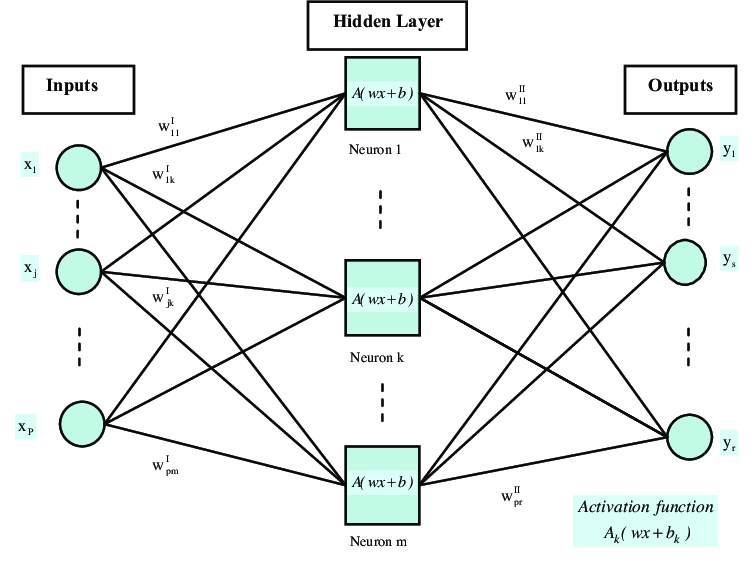
\includegraphics[width=12cm]{ANN-structure}
    \caption{A simple ANN structure with one hidden layer (Adapted from \cite{Kocadağlı})}
    \label{Figure:ANN-structure}
\end{figure}

What the network trying to do is the same as machine learning: find a function that best fits the data, so it can make predictions. The process could be expressed as:

\begin{gather}
    \mathbf{y} =\mathbf{w}^{II} \times A_k (\mathbf{w^Ix} + b^I_k)+ b^{II}
\end{gather}

The inputs fed into the network first go through a linear transformation and then map to an activation function. At last, go through a linear transformation again and output. 
By altering the parameters, it is possible to construct any curve. 

Deep learning emphasizes the use of deep neural networks, which means networks with multiple hidden layers. These networks are capable of learning complex datasets with non-intuitive 
characteristics. The depth allows the network to automatically learn features at different levels of abstraction.

Backpropagation is a key used in training deep neural networks. It is a supervised learning algorithm that adjusts the parameters $\mathbf{w}$
by propagating the error backward from the output layer to the input layer. This allows the network to update parameters to optimize predictions. 
Gradient descent is one of the backpropagation methods. Knowing the error from prediction, it measures which connection in the hidden layer.

\subsection{Activation Functions} \label{Section:activation}

The choice of activation function is vital in neural networks by introducing non-linearity into the model \cite{activation}. 
It enables the network to learn complex patterns and relationships in the data. 

\subsubsection{Rectified Linear Unit (ReLU)}

ReLU is one of the most commonly used activation functions. It replaces all negative values in the inputs with zero, which can be represented by: 
\begin{gather}
    f(x) = \mathrm{max}(0, x) 
\end{gather}

During the training, it will not activate all neurons at the same time, which gives an advantage that it is computationally efficient.
However, when $x < 0$, the gradient is zero. As training progresses, neurons may become inactive and weights fail to update.
To solve this problem, a variant of ReLU, Leaky ReLU, could be used instead. Leaky ReLU allows a small, non-zero gradient when the input is negative.

\begin{gather}
    f(x) = \mathrm{max}(\alpha x, x) 
\end{gather}

Where $\alpha$ is a small positive constant. A plot of both functions is shown in \fref{Figure:ReLUplots}

\begin{figure}[!htb]
    \centering
    \subcaptionbox{ReLU}{
        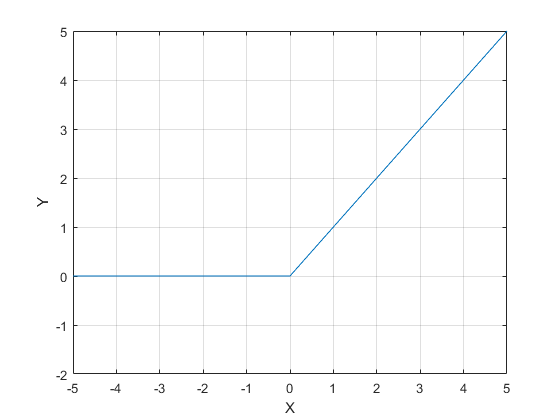
\includegraphics[width=6.5cm]{ReLU}
        \label{Figure:ReLUplots:ReLU}
    }
    \subcaptionbox{Leaky ReLU}{
        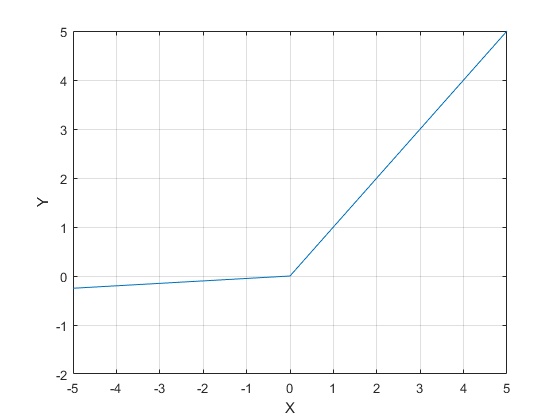
\includegraphics[width=6.5cm]{LeakyReLU}
        \label{Figure:ReLUplots:LeakyReLU}
    }
    \caption{ReLU activation functions}
    \label{Figure:ReLUplots}
\end{figure}

It is also possible to use the exponential linear units (ELU) to address the problem of inactive neurons. 
It uses $e^x-1$, which gives a similar curve, but has a small negative value at $x < 0$. 

\subsubsection{Other Functions}

There are many other activation functions such as sigmoid, hyperbolic tangent (Tanh), Softmax, etc.
Those are suitable for different purposes. For example, sigmoid have a limited output range, suitable to use before output. 
However, the curve gets too smooth at two ends, which causes a low learning efficiency. It is more used in classification problems. 

\section{Recurrent Neural Networks (RNNs)}

RNNs are a type of ANN designed for sequence data where the order of the data points is crucial \cite{lipton2015critical}. 
This makes RNN a good approach for this project. Similar to the simple ANN, RNN is constructed by multiple RNN cells. The formula of each cell is given by:

\begin{gather}
    \mathbf{h}_t = A (\mathbf{w^Ix}_t + \mathbf{w^{II}h}_{t-1} + b)
\end{gather}

Where $\mathbf{x}_t$ is the input at time $t$, $\mathbf{h}_t$ is the output at $t$, hence, $\mathbf{h}_{t-1}$ is the output at time $t-1$. 
Everything else is the same as the simple ANN. The essence of RNN is that the output of the current moment will take place in the calculation 
of the next moment as one of the inputs. \fref{Figure:RNN-structure} illustrates the idea of RNN.

\begin{figure}[!htb]
    \centering
    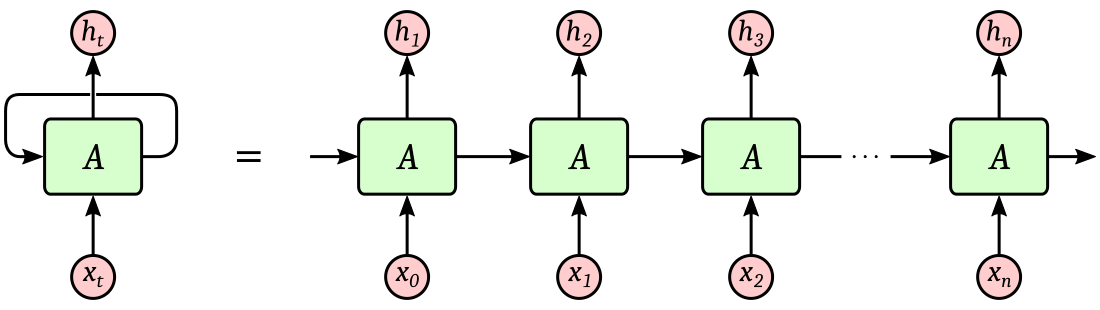
\includegraphics[width=12cm]{rnn}
    \caption{RNN as a neural network very deep in time (Adapted from \cite{rnnplot})}
    \label{Figure:RNN-structure}
\end{figure}

RNNs are susceptible to the vanishing/exploding gradient problem \cite{ribeiro2020exploding}. 
Since the RNN uses the backpropagation to minimize the cost function, and the error has been calculated from outputs going back through the network to update the weights, 
those weights in the feedback loop ($\mathbf{w_{rec}}$) are multiplied a lot of times during the backpropagation. 
If $\mathbf{w_{rec}} < 1$, the gradient will be vanishing, since it approaches 0. In contrast, If $\mathbf{w_{rec}} > 1$, then the weight will tend to be very large, i.e. exploding. 

\section{Long Short-Term Memory (LSTM)}

\begin{figure}[!htb]
    \centering
    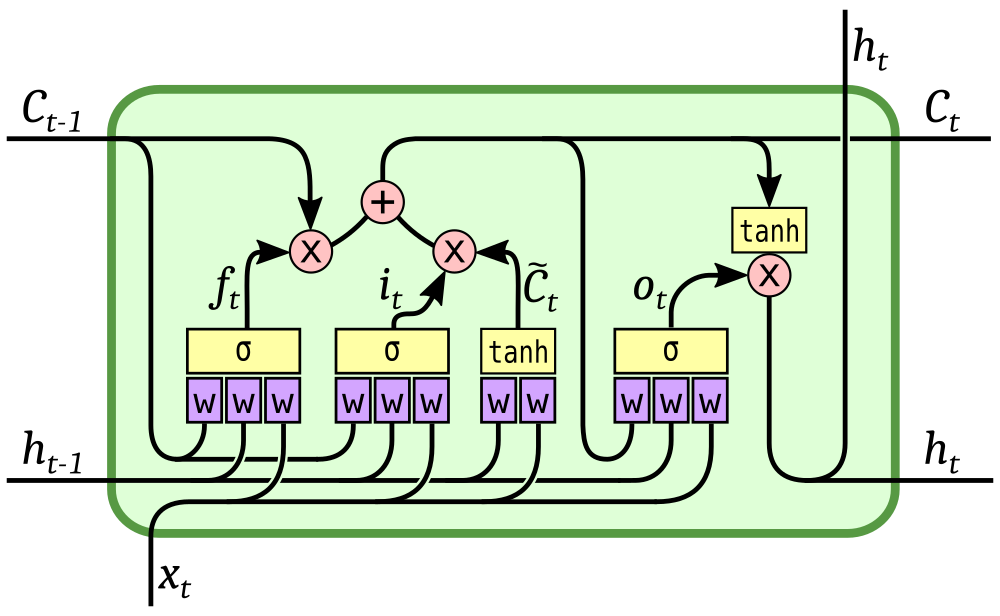
\includegraphics[width=12cm]{lstm}
    \caption{LSTM with peephole connections (Adapted from \cite{rnnplot})}
    \label{Figure:LSTM-structure}
\end{figure}

To address the vanishing/exploding gradient problem, multiple variations of RNN have been proposed. 
Long Short-Term Memory (LSTM) networks are one of the popular architectures \cite{lstm}. 
The structure of LSTM is shown in \fref{Figure:LSTM-structure}. 

The LSTM network introduces three gates to manage the weights of samples in the sequenced data. $f$ is the forget gate, $i$ is input gate, and $o$ is forget gate. 
$\sigma$ is a signoid function that gives a value between 0 and 1, which can act like a switch. 
$\mathbf{h}$ and $\mathbf{c}$ stands for hidden state and cell state. Each carries a memory path to pass down information.  
The equation of each value is given by: 

\begin{gather}
    \mathbf{i} _t=\sigma (\mathbf{w} _{xi}\mathbf{x} _t + \mathbf{w} _{hi}\mathbf{h} _{t-1} + b_i) \notag\\
    f_t=\sigma (\mathbf{w} _{xf}\mathbf{x} _t + \mathbf{w} _{hf}\mathbf{h} _{t-1} + b_f) \notag\\
    \mathbf{o} _t=\sigma (\mathbf{w} _{xo}\mathbf{x} _t + \mathbf{w} _{ho}\mathbf{h} _{t-1} + b_o) \notag\\
    \mathbf{\tilde{c} } _t=\tanh (\mathbf{w} _{xc}\mathbf{x} _t + \mathbf{w} _{hc}\mathbf{h} _{t-1} + b_c) \\
    \mathbf{c} _t=f_t \odot \mathbf{c} _{t-1} + \mathbf{i} _t \odot \mathbf{\tilde{c} } _t \notag\\
    \mathbf{h} _t=\mathbf{o} _t \odot \tanh (\mathbf{c} _t) \notag
\end{gather}

These gates, or rather sigmoid functions, let LSTM choose to ignore a sample if the current sample has been considered as not important. 
Otherwise, the LSTM will discard the information before the sample, and only retain the information of current time $t$. 

In the first version of LSTM, there is no output gate \cite{ribeiro2020exploding}, and the equations looks like this: 

\begin{gather}
    \mathbf{i} _t=\sigma (\mathbf{w} _{xi}\mathbf{x} _t + \mathbf{w} _{hi}\mathbf{h} _{t-1} + b_i) \notag\\
    f_t=\sigma (\mathbf{w} _{xf}\mathbf{x} _t + \mathbf{w} _{hf}\mathbf{h} _{t-1} + b_f) \notag\\
    \mathbf{\tilde{h} } _t=\tanh (\mathbf{w} _{xc}\mathbf{x} _t + \mathbf{w} _{hc}\mathbf{h} _{t-1} + b_c) \\
    \mathbf{h} _t=f_t \odot \mathbf{h} _{t-1} + \mathbf{i} _t \odot \mathbf{\tilde{h} } _t \notag
\end{gather}

It is clearer that in this set of equations, $\mathbf{i}$ controls the weight of short-term memories, and $f$ controls longer memories. 
Those two gates are independent. While training, it can find suitable parameters for $\mathbf{i}$ and $f$, 
which means $\mathbf{i}$ and $f$  will use different $\mathbf{x} _t$ and $\mathbf{h} _{t-1}$ to give different control strategies.

The addition of the output gate and use of $\mathbf{c}$ is to keep the longer memories more effectively. 
$\mathbf{c}$ does not exit the output gate, hence it is not affected if the current output gate is approaching 0. 
Even though the current $f$ is tend to 0, which means $\mathbf{c}_{t-1}$ has been forgotten, $\mathbf{h} _{t-1}$ still contains information about $\mathbf{c}_{t-1}$. 
This allows the long-term memories to pass down through the time sequence. 

\addtocontents{toc}{\protect\newpage}
\addtocontents{toc}{\protect\vspace*{4cm}}
%% ----------------------------------------------------------------
%% Preparation.tex
%% ---------------------------------------------------------------- 
\chapter{Data Preprocess} \label{Chapter:Preparation}

\section{Dataset Explained}

The dataset was found and downloaded on the internet \cite{Dataset}, which contains real data gathered in the city of Guiyang, China.
The traffic information was processed and integrated by collecting users' geographical locations from the navigation app anonymously in real-time. 
The dataset is separated into three datasheets. 

\begin{figure}[!htb]
    \centering
    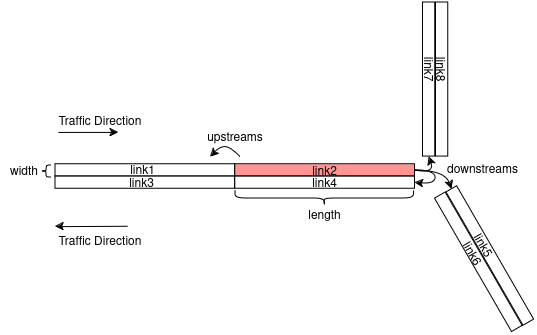
\includegraphics[width=12cm]{links}
    \caption{A diagram of links and its upstreams and downstreams}
    \label{Figure:links}
\end{figure}

In the dataset, each direction of the traffic of a road is composed of one or multiple “links”. An example of a link could be found in \fref{Figure:links}.
The first datasheet contains static information of a total of 132 links. First a few lines of the datasheet are shown in \fref{Figure:link_info}.
\verb|link_ID| is a unique string ID assigned to each link; \verb|length| and \verb|width| of the links are integer values in meters;
\verb|link_class| is the classification of the road.

\begin{figure}[!htb]
    \centering
    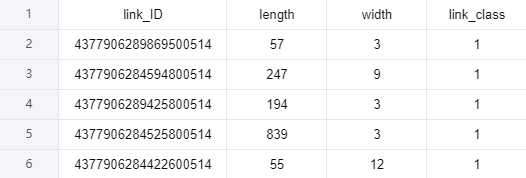
\includegraphics[width=10cm]{link info}
    \caption{First five samples of link info}
    \label{Figure:link_info}
\end{figure}

The second datasheet records the upstream and downstream relations of each link, forming the topology of the map. The headers are shown in \fref{Figure:link_top}.
\verb|in_links| records the upstream \verb|link_ID|. If there are multiple of them, a \verb|#| symbol is used to separate them. 
Similarly, \verb|out_links| records all the downstream roads. 

\begin{figure}[!htb]
    \centering
    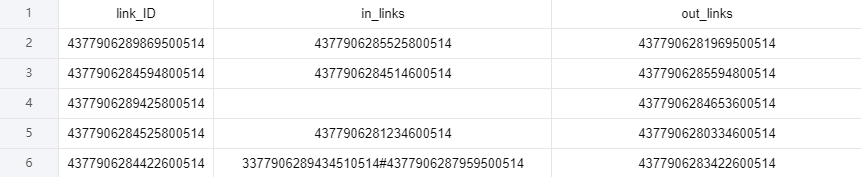
\includegraphics[width=14cm]{link top}
    \caption{First five samples of link topology}
    \label{Figure:link_top}
\end{figure}

The third datasheet is the records of the \verb|travel_time|, which is the temporal data. The data is sampled in a two-minute period.
\verb|travel_time| averages the time of vehicles that stay on the link within that two-minute time frame in seconds(\fref{Figure:records}). 
It is a float variable that has a range of values between 0 to 120. 
A higher number reflects a more congested road, by predicting \verb|travel_time|, it is able to have an idea of the traffic condition on the road.
Alongside with \verb|travel_time|, the datasheet also includes the record time interval and the date of the record. 
There are a total of 25,999,603 records, distributed from March to June of 2016 and from March to July of 2017.

\begin{figure}[!htb]
    \centering
    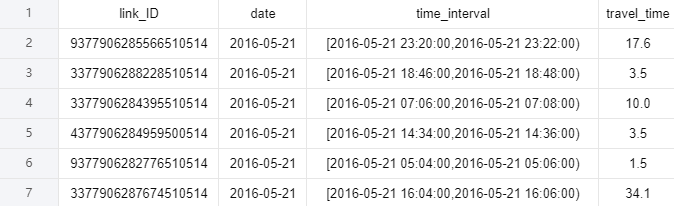
\includegraphics[width=12cm]{records}
    \caption{First six samples of records}
    \label{Figure:records}
\end{figure}

\section{Data Analysis \& Preparation}

\subsection{Static Data} \label{Section:StaticData}

\begin{figure}[!htb]
    \centering
    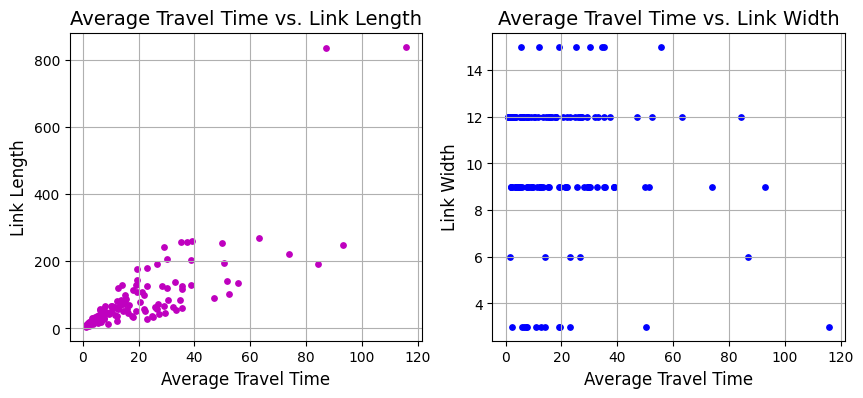
\includegraphics[width=12.5cm]{length_width_plot}
    \caption{Length \& Width vs. Average Travel Time}
    \label{Figure:length_width}
\end{figure}

All links in the dataset have a \verb|link_class| of 1, hence it is abandoned from further usage. 
The relation of the \verb|length| and \verb|width| of links and the \verb|travel_time| has been studied, and the plot is shown in \fref{Figure:length_width}.
In the plot, length has a strong positive correlation with travel time, whereas width seems to have a range of distribution.
As shown in the plot, most of the links have a length under 300 meters. Two minutes is more than enough for vehicles to pass the length. 
Hence generally the longer the links, the longer time it takes for vehicles to pass it. 
Both \verb|length| and \verb|width| can be used as features, this forms a static input shape of $\mathbb{R}^{132\times 2}$. 

\subsection{Spatial Data} \label{Section:SpatialData}

Since vehicles cannot vanish on the road, the history traffic status of upstreams of a link is highly related to its future condition. 
An adjacency matrix $\mathbf{A} \in \mathbb{R}^{132\times 132}$ is created based on the topology of the 132 links. 
Number $i$ row in $\mathbf{A}$ represent link $i$, and if the link $i$ has a downstream of $j$, then $\mathbf{A}_{ij} = 1$. 
This is the method described in Equation \ref{eq:top_adj}. 

Aside from the graph approach, it is also possible to include the spatial information by adding the travel time of the last time frame of the upstreams as features. 
There are a maximum of 4 upstreams a link can have in the given map. Hence 4 additional features are added to each sample. 
The features contain \verb|travel_time| at the last time frame of the upstream links, $0$ is initialised if not present. 

\subsection{Temporal Data} \label{Section:TemporalData}

As mentioned in \sref{Section:StaticData}, the \verb|travel_time| should be the target to predict. 
The datasheet contains other temporal information: year, month, date, and time of the day. 
\fref{Figure:day_month_year}.A illustrates that different months and years do have different average travel time, hence they could be included as features. 

The temporal features i.e. years, months, etc. are integer encoded. This might lead to the model incorrectly assuming magnitude relationships between categories. 
To eliminate this misunderstanding, one-hot encoding is used. \verb|month| is encoded into 12 features, each feature represents a month. 
On the other hand, although \verb|year| in this dataset contains only 2 values, 2016 and 2017, considering the extensibility of the model, \verb|year| stays as integer values. 

\begin{figure}[!htb]
    \centering
    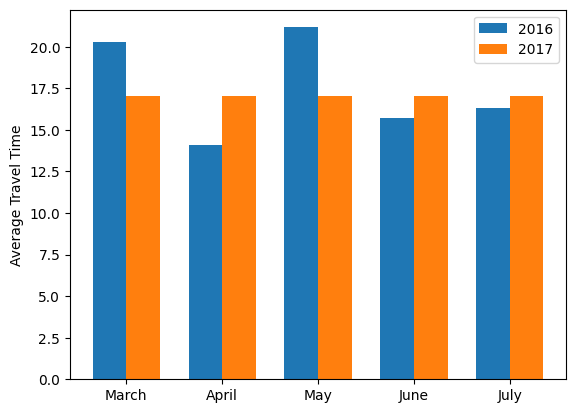
\includegraphics[width=7cm]{month year}
    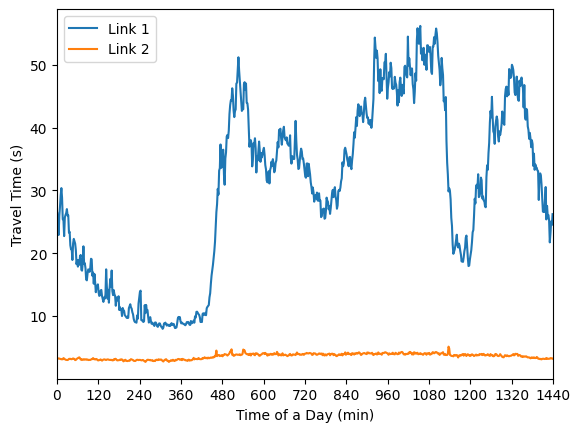
\includegraphics[width=7cm]{time of day}
    \caption{(A) Average travel time varies with different month and year; (B) Time of day vs. average travel time of two randomly choosed links}
    \label{Figure:day_month_year}
\end{figure}

The time of the day also reveals characteristics. \fref{Figure:day_month_year}. B shows the plot of two randomly chosen links.
Link1 varies a lot at different times. In contrast, Link2 gives a much flattened curve. It implies that the time of a day of different links has a different impact on the travel time.
The time of day is appropriate to be a feature. Due to the fact that the value of the time is not ordinal, the one-hot encoding should be used. 
However, this way one-hot encoding needs to create too many features that require large graphics memory in the GPU. 
To reduce the high memory consumption, weather it is rush hour is used as a substitution. 
From this plot, rush hours when the curve changes the most could be determined. 7-9 am. is considered the morning rush hour, and 5-7 pm. is the evening rush hour.

Based on the information given in the dataset, some other features can be obtained using external sources. For example, holiday and weekday information.
Weekdays are determined using \verb|datetime| library and holidays can be determined by a library called \verb|chinese_calendar|, which records the local holidays of the given dataset.

Whether it is a holiday affects people's behaviour, and weekdays are selected since some of the links reveal periodicity throughout the week. 
By plotting them with the travel time on \fref{Figure:weekday_holiday}, it can be seen that the weekdays are generally higher in terms of travel time than holidays and weekends.

\begin{figure}[!htb]
    \centering
    \subcaptionbox{Holiday (1); Working day (0)}{
        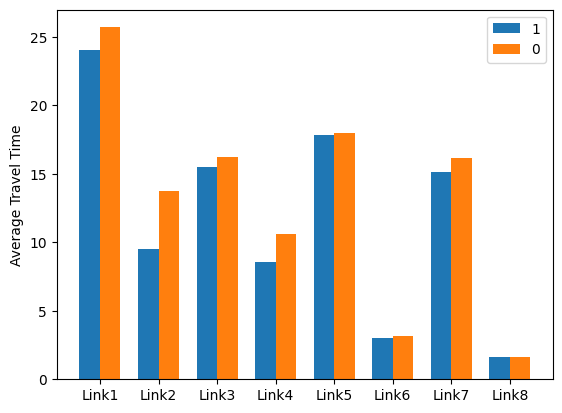
\includegraphics[width=7cm]{is holiday}
        \label{Figure:weekday_holiday:holiday}
    }
    \subcaptionbox{Weekend (1); Weekday (0)}{
        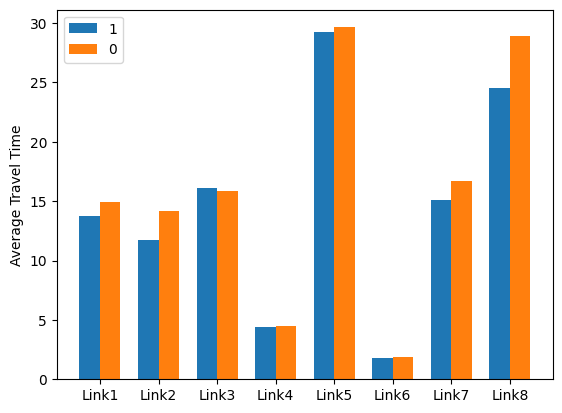
\includegraphics[width=7cm]{is weekend}
        \label{Figure:weekday_holiday:weekday}
    }
    \caption{8 randomly choosed links are used to compare (A) holiday (B) weekend with normal working day}
    \label{Figure:weekday_holiday}
\end{figure}

It has been noticed that most links have missing data at various time segments.
No matter what method is used to try to fill these missings, there will always be varying degrees of distortion.
Also in actual applications, the model is likely to encounter missing values. 
If the model does not learn how to deal with missing values, the performance in real applications may be affected.
Hence, a separate feature \verb|is_missing| telling if the sample is missing is used. Let the model learn the missing values itself. 
For samples that are missing, all other features are $0$ expect \verb|is_missing|.

\section{Train-Test Set Split}

The dataset is separated into three sets: training set, validation set, and test set. 
The whole dataset contains samples from \date{March, 1, 2016} to \date{June, 1, 2016}, and \date{March, 1, 2017} to \date{July, 1, 2017}. 
The test set includes the last 10 days of both periods. It is used to evaluate the final performance of the trained model, providing an unbiased estimate of the performance on unseen data. 
The validation set takes another 20\% of samples. It is used along with the training set while training the model. 
It helps in selecting the best-performing hyperparameters of the model, preventing overfitting. 
The samples left are the training set. This is the set that is used to train the model. It consists of features as input data along with their corresponding target labels, \verb|travel_time|.

\section{Sequence Generation}

A sequence has to be generated as input of the RNN layers. It uses a certain amount of previous samples to predict future ones. 
An hour (30 samples) of previous samples is decided to be used to predict the following half-hour (15 samples) targets. 
This will give an input dimension of $\mathbf{X} \in \mathbb{R}^{N\times S\times F}$, where $F$ is the number of features, $S = 30$ refers to the sequence length which is the 30 previous samples, and $N$ being the number of sequences that generated from the training set.
The targets, on the other hand, have a dimension of $\mathbf{Y} \in \mathbb{R}^{N\times H\times 1}$. $H = 15$ is the output length. Features expect the travel time is not included in the output sequence.

\begin{figure}[!htb]
    \centering
    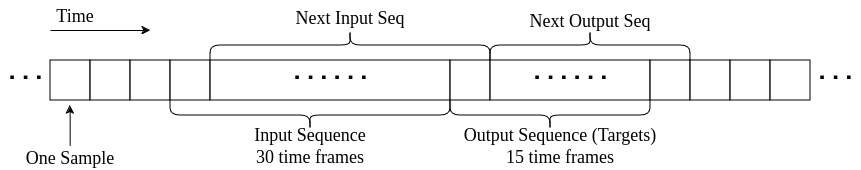
\includegraphics[width=14cm]{inout seq}
    \caption{Illustration of sequences}
    \label{Figure:inout_seq}
\end{figure}

For each different set of 45 continuous samples, a unique input sequence can be constructed. Hence for a training set continuous in time, $B$ could be calculated by:
$N = M - S - H$ where there are $M$ samples in the training set. It is worth noting that the features of the targets are not included in the input in this design. 
This may cause the model to miss some vital information about the target time frame, for example, whether the target value is missing, whether the targets are in rush hours, etc. 
In other words, when training the model with this sequence generator, it not only captures the pattern of the features on the \verb|travel_time| of target time frames but also has to capture the patterns of features and make predictions on future features.

%% ----------------------------------------------------------------
%% Designs.tex
%% ---------------------------------------------------------------- 
\chapter{Model Designs} \label{Chapter:Designs}

Tensorflow 2 with Keras API is chosen to accomplish the design of neural networks and train them.
GPU is used to accelerate the training process. Detailed development tools and versions are listed in \tref{Table:version-control}.

The process of training is to use the input data and the targets in the training set to adjust the weight vectors and make the prediction results as close as possible to the target value. 
The model will iterate through the training set a number of times. Each time is called an epoch. In theory, the performance of each traversal will be better than the last epoch. 
In each epoch, the training data is divided into batches, and each batch contains $B$ input sequences, $B$ being the batch size. 
The reason to divide it into batches is to enable GPU to do parallel training, significantly saving time consumption. 
Each batch is randomly sampled from the entire training set, which can increase the randomness of the data, and reduce the model's dependence on specific batches of data. 

The early stopping method is used throughout the training process. It is a process to monitor some indicators and stop training when a certain condition is met. 
For all the model designs, the MSE is monitored and the training will stop when the loss stops decreasing for 10 epochs. 

\section{Localised Designs}

\subsection{Pure Temporal Design}

A simple LSTM model is designed to extract temporal information. A total of 19 features for each sample are used as input. 
The static features are not included since they are constant for a single location.
\tref{Table:simplelstm-features} gives all the features used and the positions they are at. In the process of training, all the features are treated as \verb|float32|.
The types in the table are just an indication of what kind of values they might be. 

\begin{table}[!htb]
    \centering
    \begin{tabular}{c|cc|c|cc}
    \toprule
    features & position & type & features & position & type \\
    \midrule
    \verb|year| & 0 & float &  \verb|is_morning_rush_hour| & 15 & bool\\
    \verb|month| & 1-12 & bool & \verb|is_evening_rush_hour| & 16 & bool \\
    \verb|is_weekday| & 13 & bool & \verb|is_missing| & 17 & int \\
    \verb|is_workday| & 14 & bool & \verb|travel_time| & 18 & float \\
    
    \bottomrule
    \end{tabular}
    \caption{Dimensions of samples for a single link}
    \label{Table:simplelstm-features}
\end{table}

\fref{Figure:simplelstm-structure} shows the structure of the model. It is a sequential model in which each layer is connected one after another. 

\begin{figure}[!htb]
    \centering
    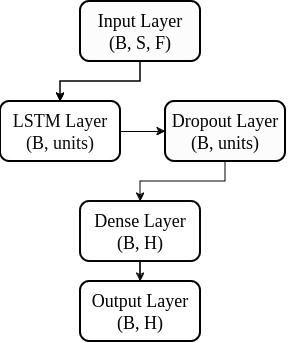
\includegraphics[width=6cm]{simplelstm-structure}
    \caption{Basic structure of the simple LSTM model, with the notes of the dimension changes}
    \label{Figure:simplelstm-structure}
\end{figure}

The input layer feeds the input sequence into the LSTM layer, with a dimension of $\mathbf{X} \in \mathbb{R}^{B\times 30\times 19}$. 
The LSTM layer with different values of units will then extract temporal information for each sequence, and change the dimension to $(B\times \mathrm{units})$.
The unit is a parameter that indicates the number of LSTM nodes in the layer. It is the length of the weight vector $\mathbf{w}$. 
Only the units in the last time frame of the sequence will be output from the LSTM layer. Those values are used to form the final targets.

To give a more powerful model, more LSTM layers could be added in series before the dropout layer. Multiple LSTM layers could increase the capacity of the model, the layer hence could capture the long-term patterns better. 
Each layer can learn feature representations at different levels of abstraction. Instead of returning the final $\mathbf{h}_t$, every output of the sequence should be returned except the last LSTM layer. 
This way, the layers could be connected sequentially.

The dropout layer randomly discards a certain amount of neurons, thereby forcing the model to have a more robust performance. 
The discard ratio can be adjusted by tuning the dropout rate. 

A dense layer is added to the end to give the correct output dimension. It is fully connected and hence has a great amount of weights to train. 
The activation function of this layer is the exponential ReLU function. 

This results in a total of 49915 trainable parameters. 
With this design, the effects on the final performance by the number of LSTM nodes, the dropout rate, and the batch size have been studied. 

\subsection{LSTM with Spatial Features}

As explained in \sref{Section:SpatialData}, features of the speed at the last time frame from the upstreams are added to the inputs. 
The resulting input dimension would now be $\mathbf{X} \in \mathbb{R}^{B\times 30\times 23}$. 
Everything else stays the same as the pure temporal model, the increase in performance by adding the spatial features would be quantified.

\section{Globalised Designs}

Another approach to predict the traffic speed is to consider the map as a whole and make predictions of every link at the same time. 
Two complicated models compared to the localised one were designed. 

The main difference between this approach from the localised designs is the sequenced data. Now the model is dealing with a total of 132 links, each link contains some statical and temporal features. 
The statical features are now in use, giving 2 additional features for every link. 
The temporal data are the features from \tref{Table:simplelstm-features}, does not change.

Combining all those together, the models now have three inputs in total: temporal inputs with a dimension of $\mathbf{X_{temp}} \in \mathbb{R}^{N\times V\times F_t}$ where $V$ stands for the number of links, $F_t$ is the feature count of the temporal data; 
statical inputs $\mathbf{X_{stat}} \in \mathbb{R}^{V\times F_s}$, where $F_s$ is the feature count of static data; and finally, the spatial inputs $\mathbf{A} \in \mathbb{R}^{V\times V}$, which is the adjacency matrix of the map. 

The model is also trained by the number of batches in each epoch, hence all three inputs need to add a dimension of batches. 
The statical and spatial inputs are broadcasted to match the dimensions.
Similar to the localised designs, the temporal inputs also need to be in sequences for LSTM layers to train. 
This makes the input shape of temporal inputs $\mathbf{X_{temp}} \in \mathbb{R}^{B\times S\times V\times F_t}$. 
This process creates a lot of duplicates of the data. Due to the memory usage restraint, a generator generates data used in each batch is used, rather than feeding the whole dataset into the model at once.  

The outputs also contain the predictions of all links. The output shape is hence $\mathbf{H} \in \mathbb{R}^{B\times H\times V}$. 
For each time frame, a prediction of the speed of every link is structured. 

\subsection{Spatio-Temporal LSTM (ST-LSTM)}

The structure of one design that can deal with spatial and temporal information is illustrated in \fref{Figure:stlstm}. 
It is a combination of the use of CNN layers and RNN layers. 

\begin{figure}[!htb]
    \centering
    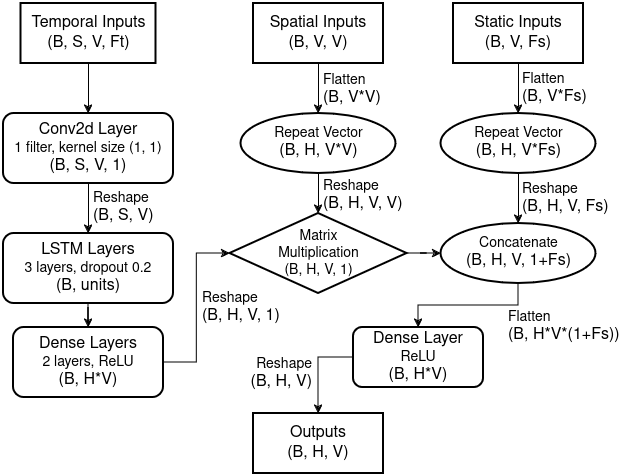
\includegraphics[width=14cm]{stlstm}
    \caption{Structure of the Spatio-Temporal LSTM design illustrated in a flowchart}
    \label{Figure:stlstm}
\end{figure}

In the sequences of the temporal data, each time frame contains two-dimensional features: $V$ and $F_t$. However, the LSTM layer can only handle one-dimensional features for one time step. 
This could be sorted by using a two-dimensional convolutional layer with 1 filter and a kernel size of (1, 1), to compress the information contained by features in $F_t$ into 1 feature. 
So now each link is related to only one feature. The LSTM layer hence can take that feature of a total of 132 links as features of the time frame. 

Now the LSTM layer is dealing with the whole map of data. It needs to be more powerful compared to ones of the localised designs. 
A three-layer LSTM sequence is used to extract temporal information. The three LSTM layers are connected sequentially, each containing 100 nodes,
The ones after using the output sequence generated from the previous layer as inputs. The final layer outputs a vector of 100 units. 

Inherit from the localised designs, two dense layers are used to match the dimension for future usage. 
The spatial inputs and static inputs are repeated first to match the target length, they are all the same across the time frames of the target. 
The processed temporal data is then multiplied with the spatial input, to merge the two data together. This is when the temporal information is combined with the spatial information.
The outcome of this stage will give a dimension of $\mathbb{R}^{B\times H\times V\times 1}$. 

The static data is then concatenated with it to extend the last dimension. Finally, a dense layer learning the statical and spatial data added is then used before the final output. 
The model contains a total of 31365780 trainable parameters, even considering 237620 parameters per link, it is still much more than the localised design. 

\subsection{GCN-LSTM}

In the ST-LSTM design, the spatial information is trained by a dense layer at the end. 
A dense layer is more effective for extracting high-level features and is suitable for data that is not affected by internal structures.
It works to extract spatial information, but it is certainly not the best choice.
Also, the input is merged into the sequenced temporal data after the extraction of temporal information by LSTM layers. 
This may cause the model to lose its vision of the spatial perspective when dealing with temporal data. 

\begin{figure}[!htb]
    \centering
    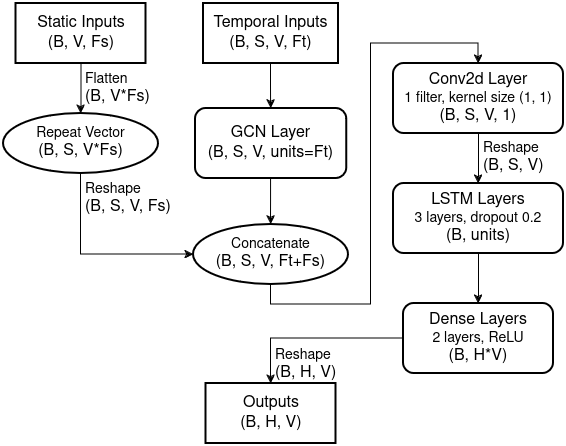
\includegraphics[width=14cm]{gcn_lstm}
    \caption{Structure of the GCN-LSTM design illustrated in a flowchart}
    \label{Figure:gcn_lstm}
\end{figure}

GCN layer is a better choice here. Since the adjacent matrix is not changing over time frames, the spatial information could be implemented into the GCN layer before training the data. 
Refering to Equation \ref{eq:gcn}, $\mathbf{D}^{-\frac{1}{2}}(\mathbf{A} + \mathbf{I})\mathbf{D}^{-\frac{1}{2}}$ is given as the model is defined.

\fref{Figure:gcn_lstm} shows the structure of the new GCN-LSTM design. 
This design is inspired by the STGCN design from \cite{Yu_2018}, which uses two temporal gated convolution layers to sandwich a spatial graph convolution layer.
In this design, the spatial inputs no longer exist since the matrix is implanted into the GCN layer. 

Before the convolutional layer and LSTM layers, the GCN layer with 19 units (which is the same amount as $F_t$) is used. 
It hence does not change the dimension of $\mathbf{X_{temp}}$, but the features are updated based on the road topology.
Along with the spatial information, the statical inputs are also merged before the extraction of the temporal information.

In this way, it should be expected to get a better performance.
In addition, there are only 2337381 trainable parameters used in total. It is significantly less than the STLSTM design, only 7.45\%.

%% ----------------------------------------------------------------
%% Results.tex
%% ---------------------------------------------------------------- 
\chapter{Model Trainings \& Results} \label{Chapter:Results}

\section{Localised Designs}

Using the simple LSTM design, the number of the LSTM units, the dropout rate, and the batch size are the parameters studied in this section. 
The model has the initial values of 100 LSTM units, a 0.2 dropout rate, and a batch size of 360. 

\subsection{Selecting LSTM Units} \label{Section:units}

Firstly, use 10, 30, 50, 100, 150, 200, and 500 LSTM units to train the model respectively, and record the MSE loss of each epoch. 
The results are plotted in \fref{Figure:simplelstm-unit}. 

\begin{figure}[!htb]
    \centering
    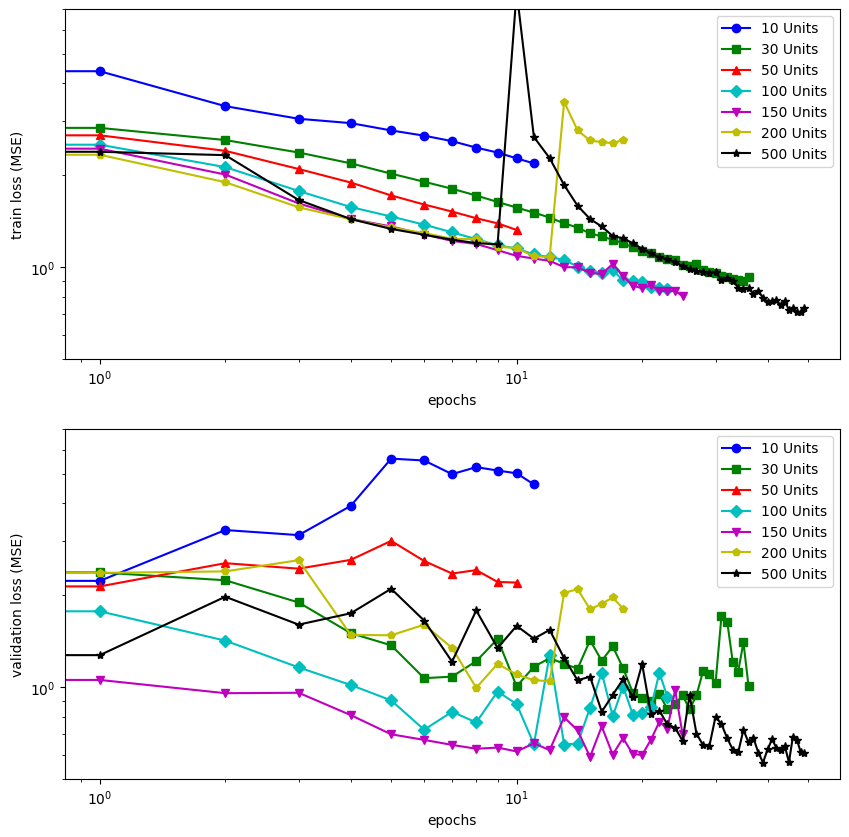
\includegraphics[width=12cm]{simplelstm-unit}
    \caption{MSE losses vs. Epochs of different numbers of LSTM units for both train and validation set}
    \label{Figure:simplelstm-unit}
\end{figure}

In general, the plot shows that the more the LSTM units, the quicker the loss reduces, and the final loss also reduces. 
In theory, larger units result in an LSTM layer with more parameters, which gives the model more capacities to be better at learning complex patterns. 
The LSTM has been designed to effectively capture longer-term dependences, more parameters could also enhance this ability of the model.
Hence, would improve the model's performance. 

Aside from the LSTM layer, an increase in LSTM units also increases the number of connections in the dense layer afterward. 
It not only increases the capability of the LSTM layer but also the dense layer. 

For both the LSTM layer and the dense layer, the time taken for each epoch increases as the number of LSTM units increases. This is straightforward since there are more variables to train each time. 
Increasing time consuming is negligible for first a few numbers of units, but it has a tendency to increase exponentially referring to \fref{Figure:simplelstm-unit-time}. 

\begin{figure}[!htb]
    \centering
    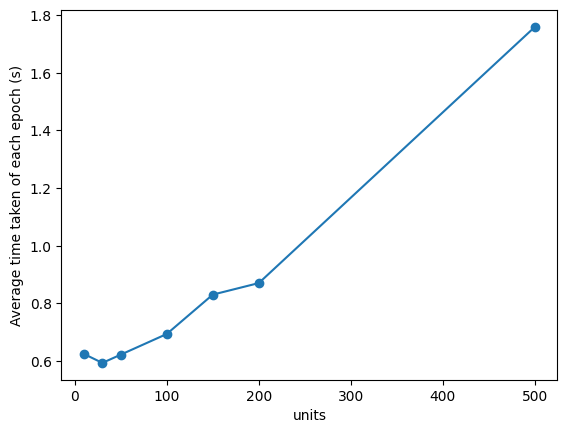
\includegraphics[width=10cm]{simplelstm-unit-time}
    \caption{Average time taken of each epoch vs. number of LSTM units}
    \label{Figure:simplelstm-unit-time}
\end{figure}

Small units like 10, clearly does not have the ability to extract common patterns of the data. The validation loss skyrocketed as the training loss slowly decreased.
The model is overfitting the training data and is not able to adapt unseen data. On the other hand, for larger numbers of units, there is a sudden rise in the training loss. 
It is a sign of the learning rate being too high. The severe fluctuations of the validation loss are another symptom.
A learning rate that is either too high or too low may lead to fluctuations in loss. 

A high learning rate may cause parameter updates too far, which could easily jump over the minimum point, and make it difficult to converge; 
while a low learning rate may cause the convergence speed to be too slow, causing the model to fall into a local minimum. 
This could be optimised by adding a learning rate scheduler in callback functions that update the learning rate dynamically.
The scheduler starts with a larger value of learning rate, 0.001. This learning rate does not change throughout the first 5 epochs.
Starting at the 6$^{th}$ epoch, the learning rate will decrease by a factor of 0.9 every epoch.

\begin{figure}[!htb]
    \centering
    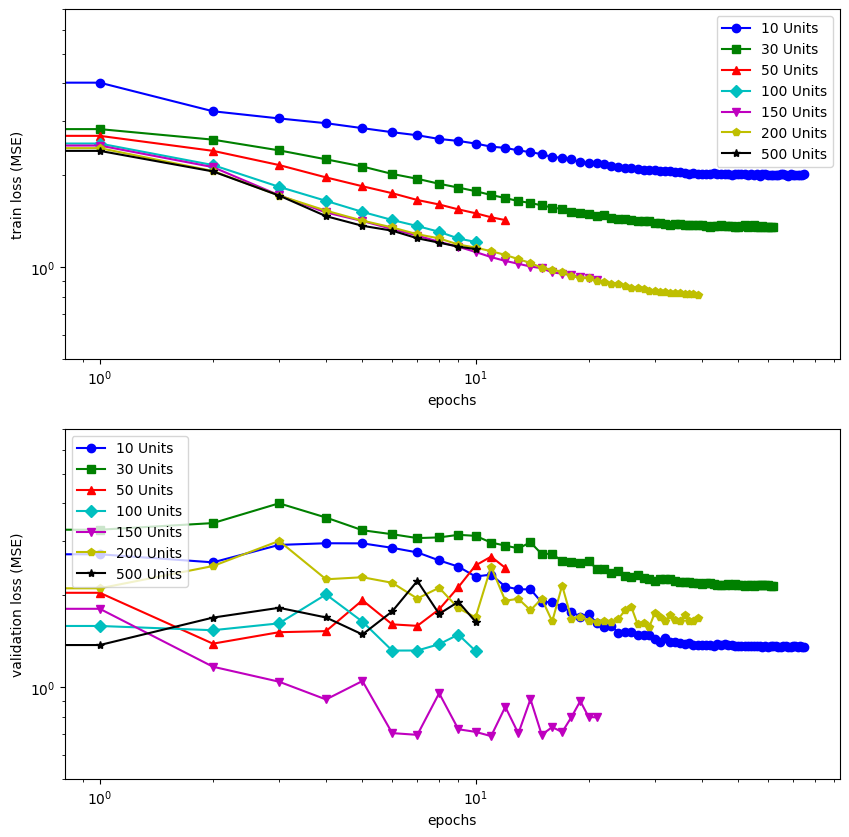
\includegraphics[width=14cm]{simplelstm-unit-lr}
    \caption{MSE losses vs. Epochs of different numbers of LSTM units with the learning rate scheduler}
    \label{Figure:simplelstm-unit-lr}
\end{figure}

After applying the learning rate scheduler, the results are shown in \fref{Figure:simplelstm-unit-lr}. 
This time the curves of both train losses and validation losses are smoother, and there is no sudden rise in training loss anymore. The largest fluctuations are at about 5$^{th}$ to 10$^{th}$ epoch, which is the starting point of the learning rate starts decreasing. 
This tells that the scheduler indeed improves the model as expected. 

For larger numbers of units, the training loss does not improve since 100 LSTM units. Some of them end earlier due to there being no significant drop in validation loss. 
This implies that it is the best performance this architecture given the same input can reach. 
On the other hand, 10, 30, and 50 units underfit the data, the losses are high in both training and validation. 

It has been noticed that each time the curve of the training and validation loss over epochs is different, especially for the validation set. Even the final validation loss is different every time the model. 
This is due to several reasons. Firstly, at the beginning of training, model parameters are initialised randomly. Therefore, even if the same architecture and hyperparameters are used, the initial state of the model is different, which will result in different training outcomes. 
Secondly, in each epoch, the model is updated based on a different batch of data. The sequences in each batch are randomly selected, which will lead to different perturbations for each training. This affects the updated trajectory of the model.
150 units are chosen due to it gives more stable results without having a massive increase in time consumption.

\subsection{Selecting Dropout Rates}

\begin{figure}[!htb]
    \centering
    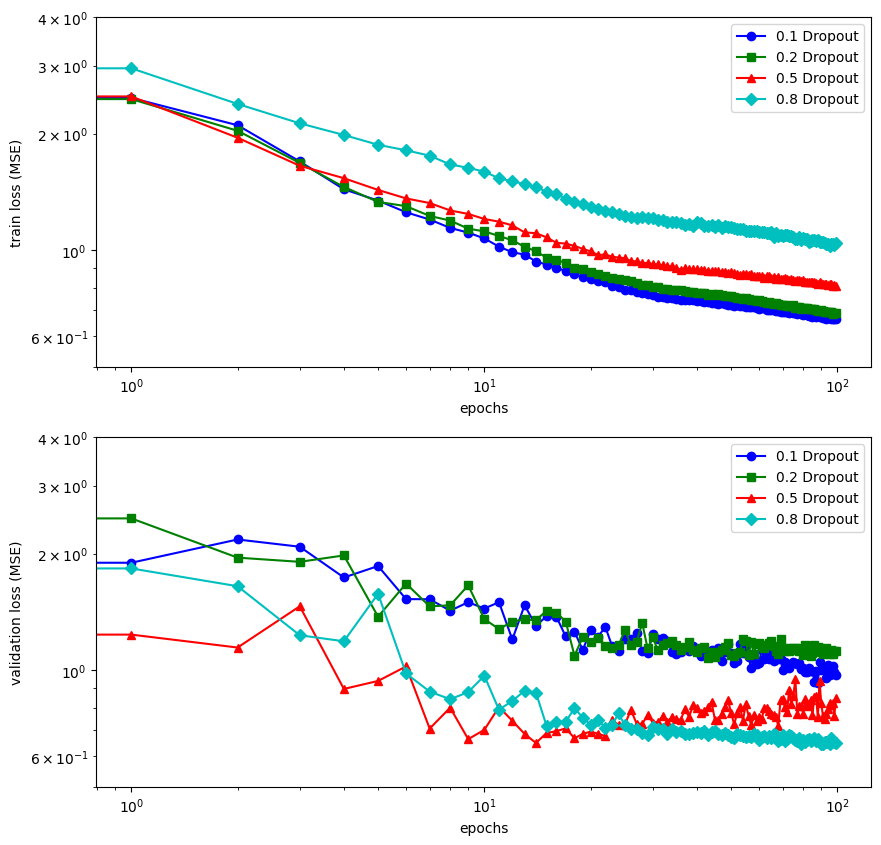
\includegraphics[width=12cm]{simplelstm-dropout}
    \caption{MSE losses vs. Epochs of different dropout rates for both train and validation set}
    \label{Figure:simplelstm-dropout}
\end{figure}

The dropout rates used in this study are 0.1, 0.2, 0.5 and 0.8. Each takes out 10\%, 20\%, 50\%, and 80\% nodes from the network. 
This is designed to prevent overfitting, hence the early stopping strategy is not used to have a better view of the effects caused by the dropout rate.
\fref{Figure:simplelstm-dropout} contains the results of them.

A higher dropout rate can more strongly reduce the overfitting of the model. It discards more nodes in the network, making the network less dependent on specific nodes.
However, a higher dropout rate also reduces the capacity of the model and causes the performance of the training set to decrease. 
On the plot, the lowest dropout rates (0.1 and 0.2) give the lowest training loss, whereas the validation loss of them is higher. 

An appropriate dropout rate is often a trade-off between overfitting and underfitting, thereby improving the overall performance of the model. 
The dropout rate of 0.5 gives roughly the same training and validation loss, it is hence the best choice.

\subsection{Selecting Batch Sizes}

Batch sizes are chosen from 10, 30, 120, 360, 720, and 1440. A large batch size could improve the training speed because each parameter update requires less calculation. 
Using a larger batch size allows the process of gradient descent to parallelise the computation to a greater extent because the sequences could be split across different computation units on the GPU and computed at the same time. 
\fref{Figure:simplelstm-batchsize-time} shows an inverse proportional relationship between the time taken for one epoch and the batch size. 

\begin{figure}[!htb]
    \centering
    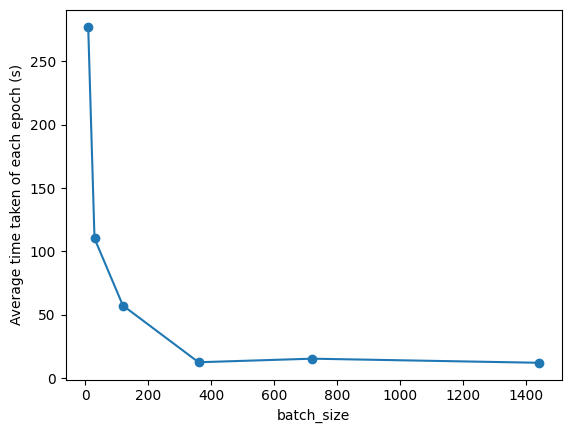
\includegraphics[width=10cm]{simplelstm-batchsize-time}
    \caption{Average time taken of each epoch vs. batch sizes}
    \label{Figure:simplelstm-batchsize-time}
\end{figure}

Different batch sizes may require different learning rates for optimal performance. Typically, larger batch sizes allow for larger learning rates, while smaller batch sizes may require smaller learning rates to avoid exploding or vanishing gradient problems.
To prevent overfitting, the learning rate scheduler explained in \sref{Section:units} and the early stopping strategy are applied. \fref{Figure:simplelstm-batchsize} gives the resulting losses of different batch sizes. 

\begin{figure}[!htb]
    \centering
    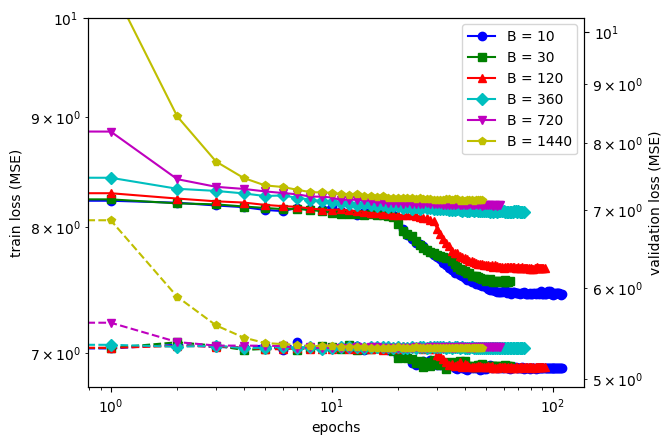
\includegraphics[width=13cm]{simplelstm-batchsize-lr}
    \caption{MSE losses vs. Epochs of different batch sizes for both train and validation set}
    \label{Figure:simplelstm-batchsize}
\end{figure}

In general, the number of iterations required to run an epoch is reduced as the batch size increases. To achieve the same accuracy, more epochs are needed. 
Memory usage is also a key factor when selecting the batch size. Smaller batch sizes can reduce memory consumption because fewer intermediate results need to be stored for each batch. 

A larger batch size can improve the stability of the model and reduce the randomness of parameter updates. 
However, if the batch size is too large, it may cause the model to fall into a local minimum and be difficult to escape.
In the experiment, batch sizes beyond 120 fall into a local minimum, in contrast, small batch sizes have a significant drop during later epochs. 
The drop happened both in train loss and validation loss, showing that this is indeed a better performance rather than overfitting. 

\subsection{Addition of Spatial Features}

By adding the spatial features, with 150 LSTM units, 0.5 dropout rate, 120 batch size, and the implementation of a learning rate scheduler, the training loss of the model drops significantly. 
A plot comparing the previous pure temporal model and the new model is presented in \fref{Figure:spatiallstm}. Both models used the same set of hyperparameters.

\begin{figure}[!htb]
    \centering
    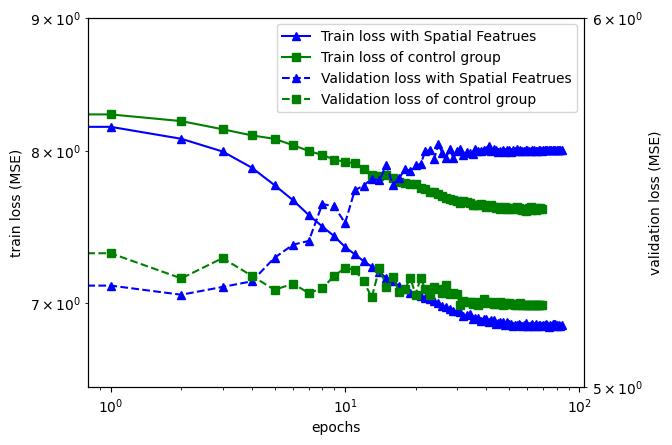
\includegraphics[width=13cm]{spatiallstm}
    \caption{MSE losses vs. Epochs comparing the pure temporal model with the addition of spatial features}
    \label{Figure:spatiallstm}
\end{figure}

The spatial features bring a 10\% reduction in the final train loss, this is significant compared to the difference in previous experiments. 
The validation loss, on the other hand, increases in later epochs, where the pure temporal design does not. 
Any feature change would affect the choice of hyperparameters, hence the process that has been done towards the pure temporal model should be done again. 

\begin{figure}[!htb]
    \centering
    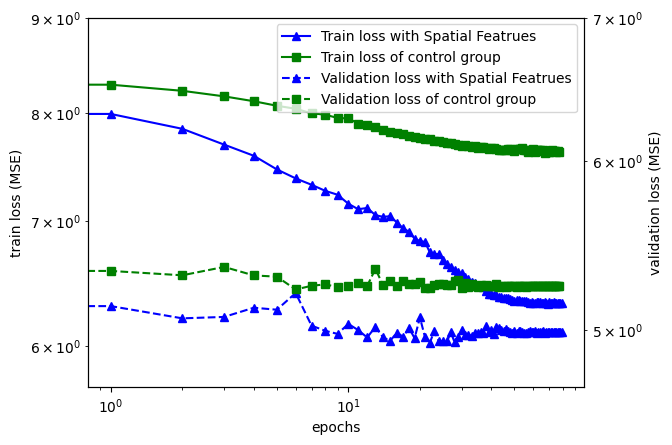
\includegraphics[width=13cm]{spatiallstm-final}
    \caption{MSE losses vs. Epochs comparing the pure temporal model with the addition of spatial features}
    \label{Figure:spatiallstm-final}
\end{figure}

By choosing appropriate hyperparameters, namely 200 LSTM units, 0.2 dropout rate, and 120 batch size, the training loss  reduced 20\% from the control group, without a raise of validation loss. 
The graph has been plotted in \fref{Figure:spatiallstm-final}.
This result shows a close relationship between the current speed of a link and the previous values of its upstreams.
The new features provide a better representation of the data, making the model easier to learn the patterns and the structure. 

Beyond this comparison, the stability of the model is explored. 
8 randomly picked links are trained using the above settings, and the MAPE is used instead of MSE. 
This is because the MAPE focuses on the relative difference, making the loss comparable between different links. 
\tref{Table:spatiallstm-links} shows the results. 

\begin{table}[!htb]
    \centering
    \begin{tabular}{c|cccccccc}
    \toprule
    ID & 118 & 36 & 47 & 88 & 114 & 70 & 21 & 74 \\
    \midrule
    Train MAPE & 72.45 & 78.88 & 78.15 & 78.88 & 79.55 & 78.39 & 77.61 & 70.22 \\
    Val MAPE & 76.25 & 79.05 & 78.73 & 79.50 & 79.83 & 79.83 & 78.76 & 80.98 \\
    \bottomrule
    \end{tabular}
    \caption{Trian and validation MAPE loss of 8 randomly picked links}
    \label{Table:spatiallstm-links}
\end{table}

The result does show a good stability of the model. The train loss varies not much in the range between 70 to 80. 
The difference is caused by the number of upstreams the link has. There are four features representing the speed in the upstreams. 
For the links only contain one or even no upstreams, such features are wasted. 
The above discussion has proven that such features have a positive impact on its performance, different links may benefit differently from these features. 

Also, based on the analysis of data in \sref{Section:TemporalData}, each link seems to have a unique distribution of data. 
Even if the data is similar, the model is more sensitive to certain features, and the importance of these features may differ in different links. 

\section{Globalised Designs}

\subsection{ST-LSTM}

Different from the localised designs, the ST-LSTM model minimise the loss by only using two epochs. Every time the loss reaches its minimum at the second epoch. 
It can be a good sign that the model has adapted well to the training set. The characteristics of data are learned in a short training period. 
Conversely, it can also be a sign of underfitting, that the model only captures the simple patterns of the data, and cannot further improve.

Instead of giving the whole training set and validation set to the model, those two sets are given by sequence generators. 
A total of three generators responsible for the training, validation, and test set were used, which means the data were separated before the sequences formed. 
This allows the training and validation set to separate completely. 

By tuning the batch size, the training and test loss stays the same, however, the validation loss increases as the batch size increases. 
The results are gathered in \tref{Table:stlstm-batchsize}. The validation loss increase is as expected since a larger batch size introduces more noise and makes the generalisation ability of the model decrease. 
The training loss, on the other hand, seems to fall into a local minimum and cannot escape. It is a sign of underfitting. 

\begin{table}[!htb]
    \centering
    \begin{tabular}{c|ccccc}
    \toprule
    B & 120 & 360 & 720 & 1440 & 5040 \\
    \midrule
    Train MSE & 1.8701e-04 & 1.8701e-04 & 1.8701e-04 & 1.8701e-04 & 1.8701e-04 \\
    Val MSE & 4.7873e-05 & 1.1068e-04 & 2.22036e-04 & 3.2226e-04 & 3.7096e-04 \\
    Test MSE & 2.2528e-04 & 2.2528e-04 & 2.2528e-04 & 2.2528e-04 & 2.2528e-04 \\
    \bottomrule
    \end{tabular}
    \caption{Minimum MSE losses vs. Batch sizes of ST-LSTM model}
    \label{Table:stlstm-batchsize}
\end{table}

This model can be considered as unsuccessful, the structure of the model designed is not suitable for the problem. 
To improve its performance, it is reasonable to change the architecture. 

\subsection{GCN-LSTM}

\begin{figure}[!htb]
    \centering
    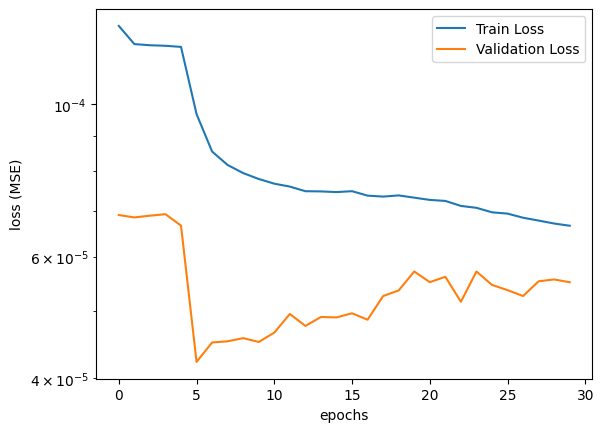
\includegraphics[width=12cm]{gcnlstm_loss}
    \caption{MSE losses vs. Epochs of GCN-LSTM model}
    \label{Figure:gcnlstm_loss}
\end{figure}

The model easily overcomes the local minimum point and trains further down the gradient. 
The performance has been improved by using the GCN layer. The path of the losses over epochs is shown in \fref{Figure:gcnlstm_loss}.

%% ----------------------------------------------------------------
%% Evaluation.tex
%% ---------------------------------------------------------------- 
\chapter{Evaluation} \label{Chapter:Evaluation}

\section{Localised Design}

The test set is fed into the trained localised model to give a general sense of how well did the model predict. 
By collecting all of the predictions together, predictions and the actual target values are plotted in \fref{Figure:eva_all}.
The graph shows a good prediction in long-term trends of the travel time, yet there are some biases. 

In the actual values, there are large fluctuations of values, these rapid changes have not been well predicted by the model. 
The values predicted are rather conservative, focusing more on the long-term trends, and tend to ignore the high-frequency fluctuations. 

\begin{figure}[!htb]
    \centering
    \subcaptionbox{Half of the test set}{
        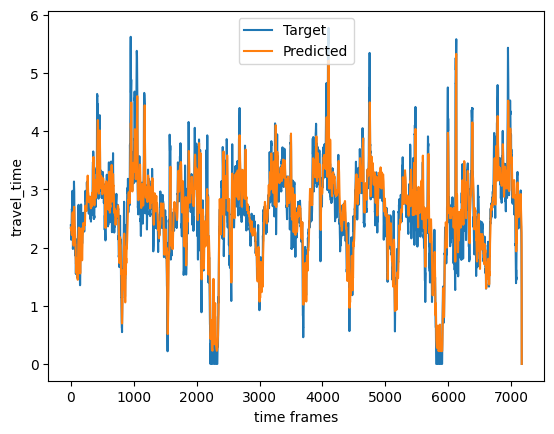
\includegraphics[width=0.48\linewidth]{eva_whole}
        \label{Figure:eva_whole}
    }
    \subcaptionbox{One day}{
        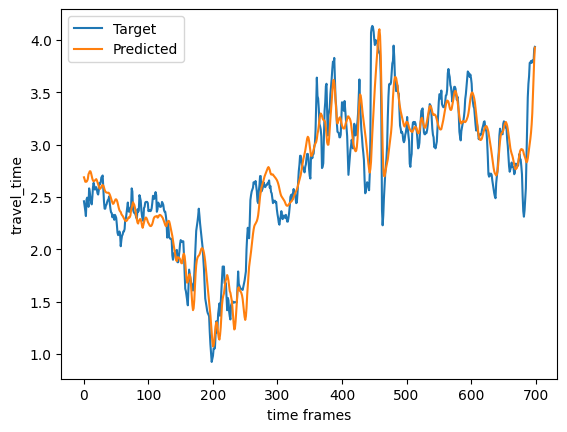
\includegraphics[width=0.48\linewidth]{eva_local}
        \label{Figure:eva_local}
    }
    \caption{Predictions from the localised design joined together compared with the actual values}
    \label{Figure:eva_all}
\end{figure}

Due to the fact that the model only predicts the next 15 minutes in advance, such a graph does not tell much about the situation to use the model.
Instead, each predictions are plotted individually with the true values. Some prepresentative examples are shown in \fref{Figure:predict}.
The first 30 data points are the inputs that feed into the model, after that comes the predictions. 
Generally, the predictions show a smooth curve that has a starting point very close to the last time frame in the inputs. 
The first few data points predicted are more accurate compared to the later ones.

\fref{Figure:fault} is an example of a prediction that has a trend that completely does not agree with the actual values. 
This is a fault prediction that happens more frequently when there is a significant increase in travel time in a short period. 
This may be due to unaccounted-for external factors and unexpected events, such as accidents. This does affect the applications of the model, like a navigation application. 
Predictions like this will affect the decision made on selecting roads and the expected time taken calculated. 

\begin{figure}[!htb]
    \centering
    \subfloat[Fault prediction\label{Figure:fault}]{
        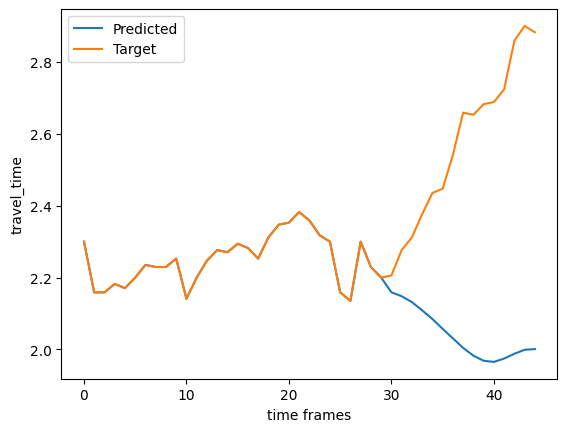
\includegraphics[width=0.48\linewidth]{eva_1}
    }
    \subfloat[Correct trends with conservative values\label{Figure:trends}]
    {
        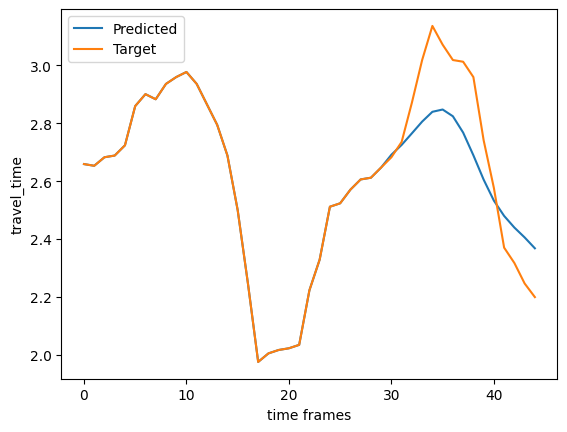
\includegraphics[width=0.48\linewidth]{eva_2}
    }
    
    \subfloat[Correct trends and values\label{Figure:correct}]{
        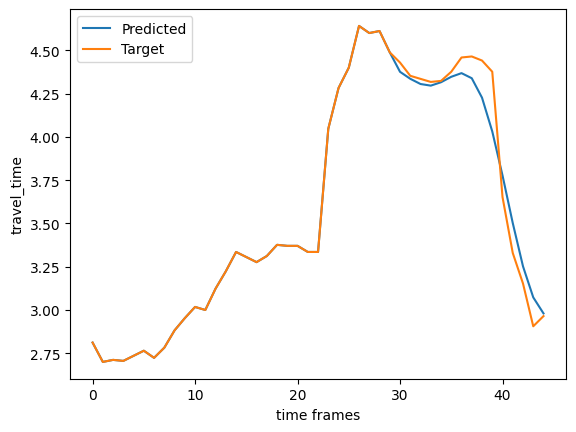
\includegraphics[width=0.48\linewidth]{eva_3}
    }
    \subfloat[Sudden change in values\label{Figure:change}]
    {
        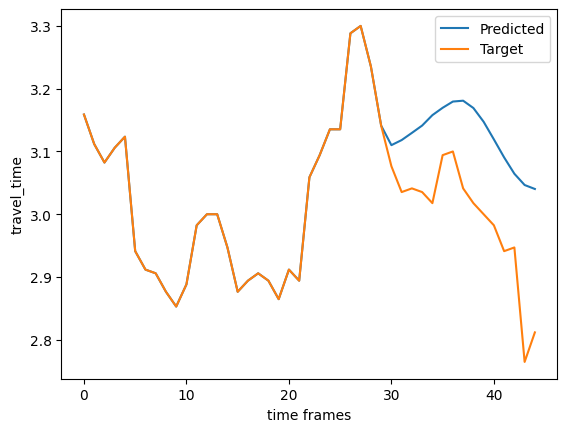
\includegraphics[width=0.48\linewidth]{eva_4}
    }
    \caption{Representative predictions in the test set}
    \label{Figure:predict}
\end{figure}

The prediction of \fref{Figure:trends} predicts the trend correctly but with a lower amplitude. 
The LSTM model generally has the nature of smoothness, which predicts noises and sudden changes relatively stably. 
It implies that the model mainly learns the general trends and cyclical changes in the data, but fails to fully capture the sudden changes in the real values. 
Also, the model may filter out some of the fluctuations as noise or outliers, which also makes the predicted values relatively smooth. 

\fref{Figure:change} have a similar condition when there is a sudden change. This time the change is given in the input sequence. 
The prediction shows a correct trend but the values are closer to the value of the last of the input sequence. 
As long as the the trend is correctly predicted, it will be fine to use since it will not affect much on decision makings. 

\fref{Figure:correct} gives an accurate prediction that it correctly predicts the trend and values. 
This is an ideal situation. These accurate predictions happen more when there is a drop in travel time. 
This may be because the characteristics of the drop are clearer than a rise in travel time in the dataset. The model successfully captures the pattern and makes good predictions. 

\section{Globalised Design}

The predictions of a single link using the GCN-LSTM model are worse compared to the localised design. 
The benefit of it is that it predicts a total of 132 links together at once. 
\fref{Figure:eva_global} shows the one-day predictions of one of the links compared with the targets.

\begin{figure}[!htb]
    \centering
    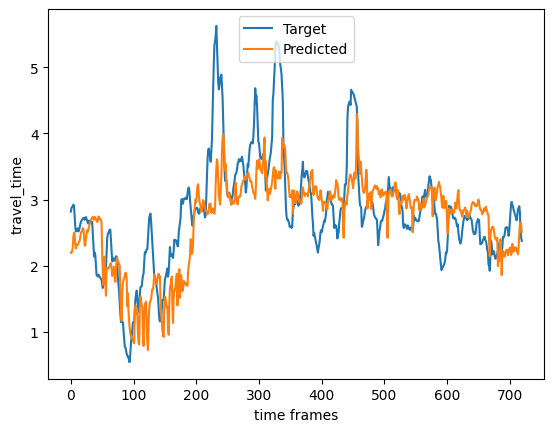
\includegraphics[width=11cm]{eva_global}
    \caption{Predictions of one link from the GCN-LSTM model joined together compared with the actual values}
    \label{Figure:eva_global}
\end{figure}

The predictions are still not far from the actual values but are a lot more off than the localised ones. 
The predictions seem lagging behind, it needs some time to adapt the jumps of the actual values. This shows that the model does not have a good ability to predict the sudden changes. 
The LSTM layers are not able to handle all links at the same time to give the same level of accuracy as for only one link.

The current performance of the GCN-LSTM model with inputs used is not ideal to be used in applications that require accurate predictions in a short period of time.
There are many more parameters and selections that could be made to optimise the performance of the model which have not been covered in the project. 

%% ----------------------------------------------------------------
%% Conclusion.tex
%% ----------------------------------------------------------------
\chapter{Conclusion \& Proposal} \label{Chapter:Conclusion}

\section{Conclusion}

Both localised and globalised designs showed their ability to predict future travel times based on historical data. 
The localised one gives a more accurate prediction focusing on a single location, whereas the globalised design uses less time and computational power to predict a whole area. 

The hyperparameter optimisation such as the batch size, and learning rate do affect the final performance of the model, but not as much as the input features and the overall structures of the model. 

Both architectures were designed with high flexibility. 
Adding or removing features will not break the models. In fact, choosing appropriate features would have a great boost in the performance of models. 
Different cities and areas may have different information collected, features could be selected based on specific locations. 
The performance could be enhanced by having a shorter time frame, which allows the model to learn the patterns of shorter periods of time. 
The information on traffic lights, accidents, and the number of vehicles would be critical to include in the inputs to further improve the performance. 
The target to predict is the travel time. However, no matter what value is given, including the average speed of vehicles, the number of vehicles on the road, etc., 
the architectures are expected to work in the same way. 

The prediction could be used as input to predict travel times in further future, however, this would give an increasingly worse prediction.

\section{Project Management}

It was a challenge to come up with a plan for this project at the start when every topic and section related to the project required study and further research. 
Different architectures to be learnt, and libraries for codes to be familiar with.
There was no good enough view of the big picture when stating the goals, and hence some of the goals and scopes have changed as progress. 
Faults, misunderstandings, and better approaches come up while designing and training models and some of them require redoing the designs completely. 
The plan has been reconsidered every time it happens.
The Gantt chart is shown in \fref{Figure:gantt}. The expected and actual progress differ significantly as seen in the Gantt chart. 

Some tasks are added to the project halfway through, and also tasks are abandoned. This was a risky move since it would change the plan for every task afterward. 
The new designs added took longer time to optimise and train than expected, which led to insufficient time to make the pathfinding algorithm based on the outputs of the models. 
It would be better if it is decided to stick with the plan, which will achieve the goals stated to a higher extent. 

Jupyter notebook is used to code with, which enables to change parameters and alter structures without rerunning the whole process. 
Git is used as version control. It makes backtracking easier. Different libraries were tried and different operating systems were prepared to ensure the platform of designing is working. 

The project brief states the issue "Assuming that an accident has occurred at a certain location, is there a way to accurately anticipate the resulting traffic conditions on the adjacent roads?"
However, due to the fact that a traffic dataset with information on accidents has not been found, there is no way that predictions are not able to reflect accidents. 

\section{Future Work}

\begin{itemize}
    \item Another dataset could be used to train the model. This would give an indication of the universality of the architecture. The ones containing information about accidents and traffic lights are preferred, due to they could potentially enhance performance. 
    \item The hyperparameters require a great deal of time and effort to optimise, tools such as Bayesian optimisation, grid search, etc. could be used to automate the optimisation process. 
    \item Different lengths of the input and output sequences could be considered. The effect of amount of historical data given to the model would potentially affect the performance of the model. 
    \item The structure of the input sequence could be optimised to include some features of the target time frames. Most of the features such as the date, time, and holidays are known values, and including them would result in a better performance. 
\end{itemize}


%% ------------------ BACK MATTER ORGANISATION -------------------

\bibliographystyle{plainnat}
\bibliography{UOS}

\appendix
%% ----------------------------------------------------------------
%% AppendixA.tex
%% ---------------------------------------------------------------- 
% \chapter{Project Brief} \label{Appendix:brief}

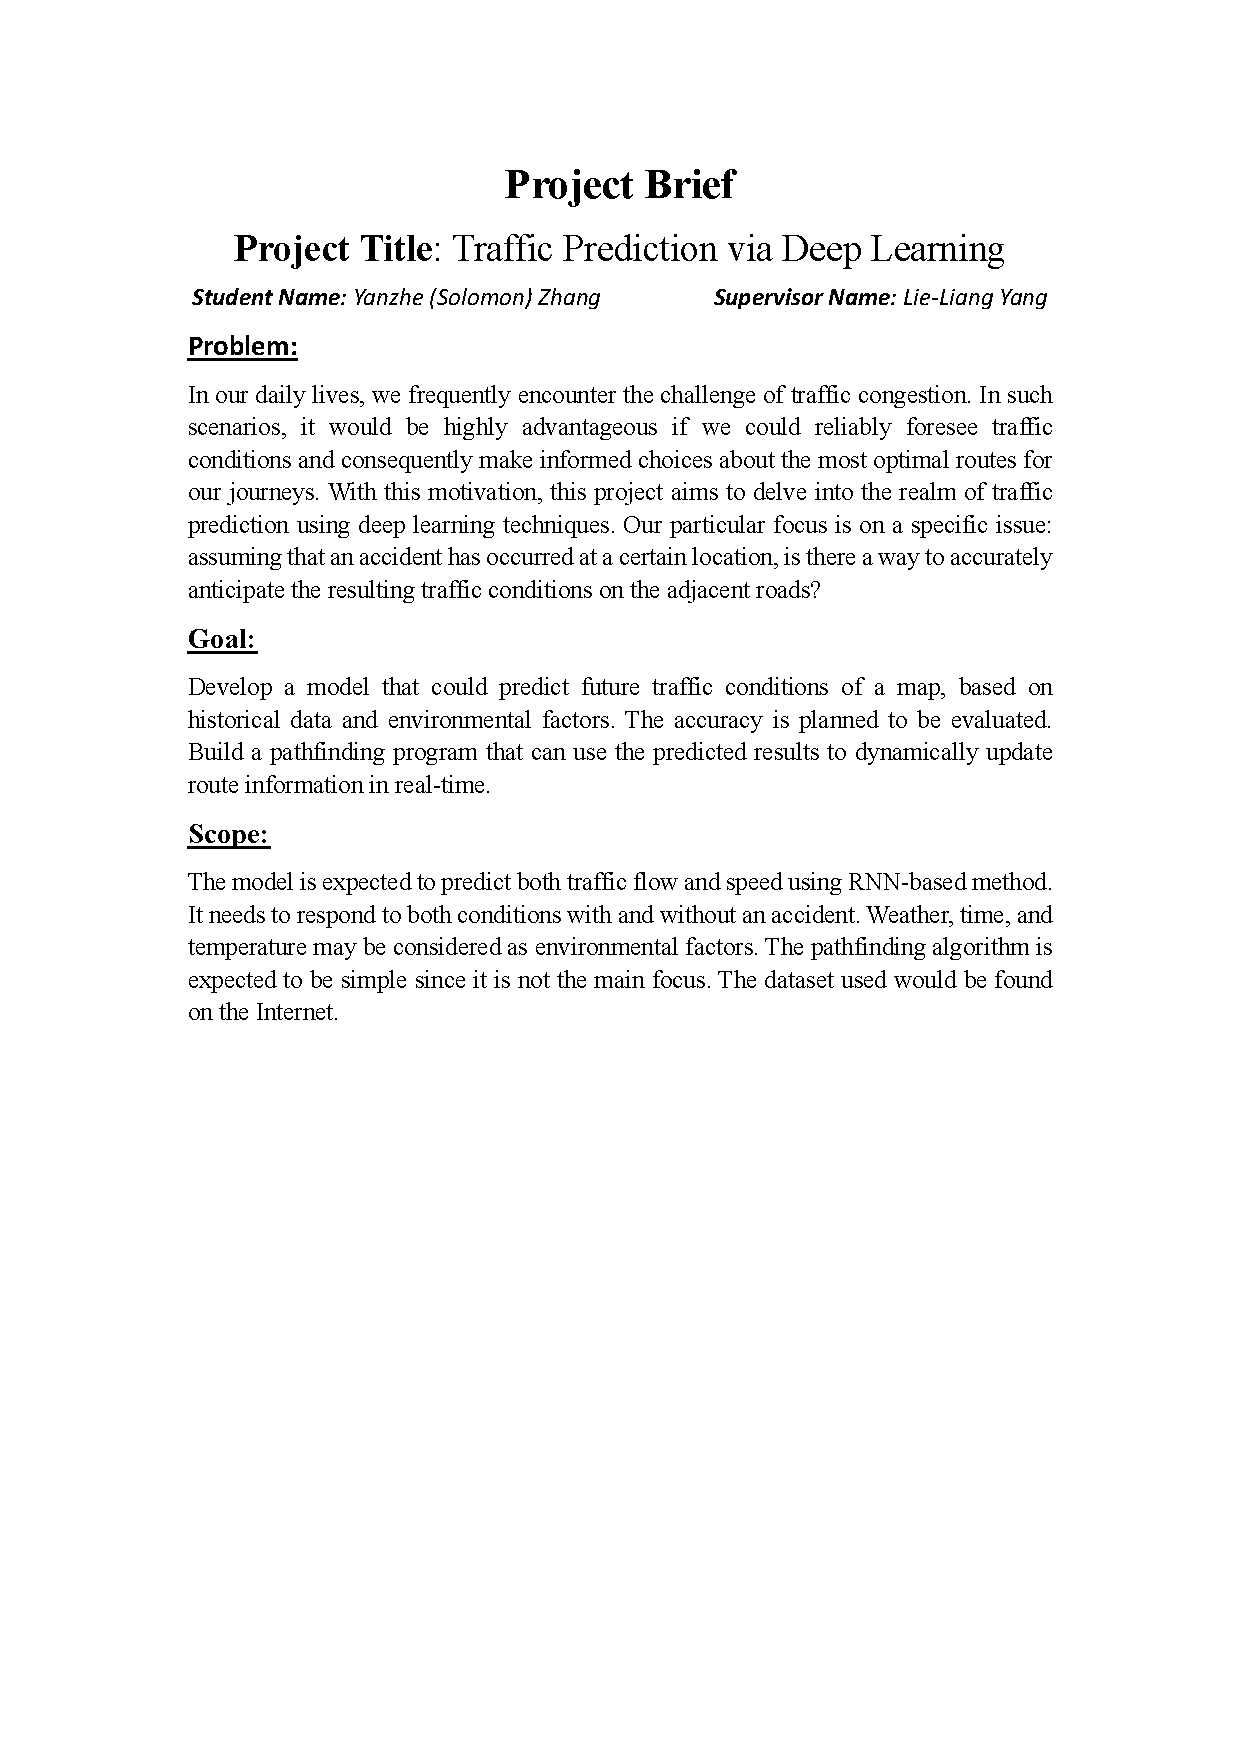
\includepdf[pages=1, scale=0.8, pagecommand={\chapter{Project Brief} \label{Appendix:brief}}, trim=2cm 12cm 2cm 1cm, clip=true]{Project Brief.pdf}

%% ----------------------------------------------------------------
%% AppendixB.tex
%% ---------------------------------------------------------------- 
\chapter{Tables} \label{Appendix:tables}

\begin{table}[!htb]
    \centering
    \begin{tabular}{|l|l|}
    \toprule
    Tools & Version \\
    \midrule
    CPU & 13th Gen Intel\textregistered Core\textsuperscript{TM} i7-13700KF $\times$ 24\\
    GPU & NVIDIA GeForce RTX 4070 Ti \\
    GPU Driver & NVIDIA UNIX x86\_64 Kernel Module 535.171.04 \\
    CUDA & 12.2 \\
    cuDNN & 8.9 \\
    Operating System & Ubuntu 22.04.4 LTS 64-bits \\
    Clang & 16.0.0 \\
    Python & 3.10.12 \\
    Tensorflow & 2.15.0.post1 \\
    numpy & 1.24.4 \\
    \bottomrule
    \end{tabular}
    \caption{Development tools and version requirements}
    \label{Table:version-control}
\end{table}

\begin{landscape}

\begin{figure}[!htb]
    \centering
    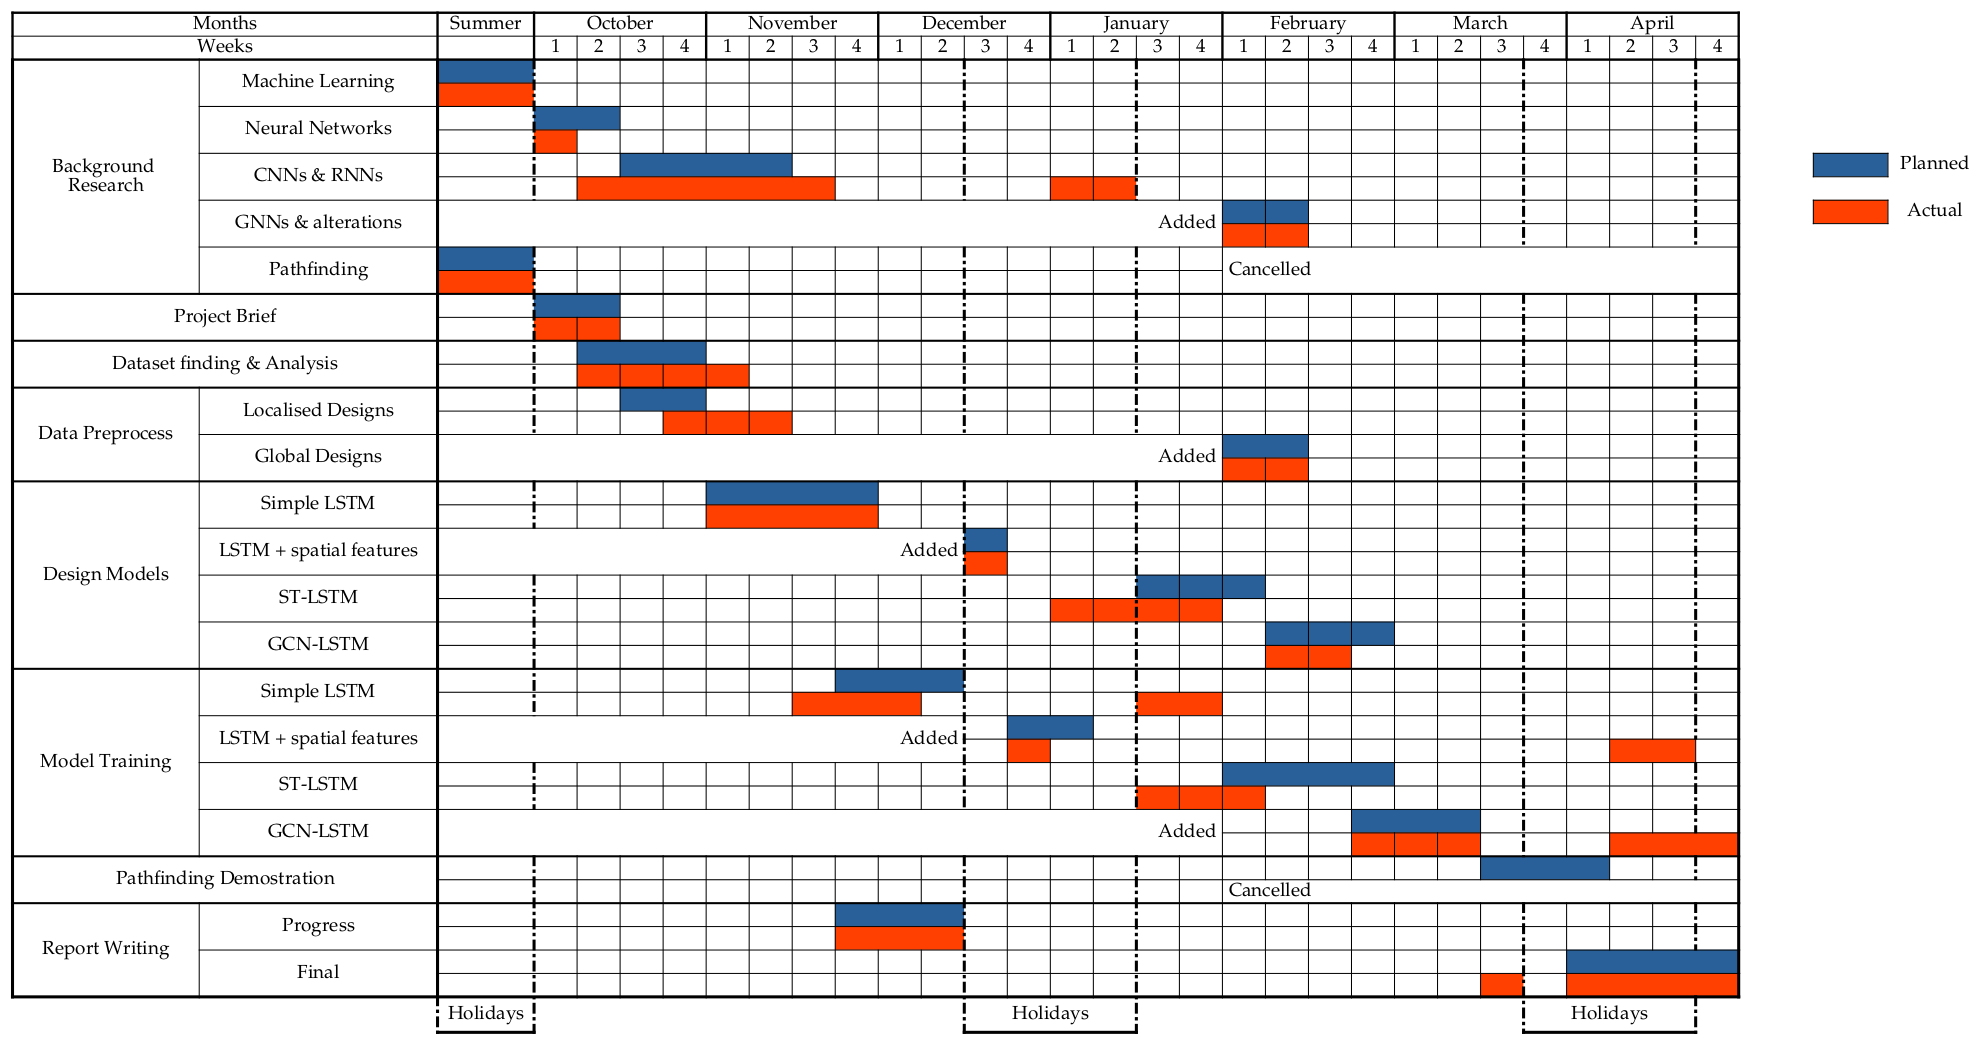
\includegraphics[width=24cm]{Gantt Chart}
    \caption{Gantt Chart with planned progress and actual progress}
    \label{Figure:gantt}
\end{figure}

\end{landscape}

\backmatter

% \chapter{Glossary [if relevant]}

% \chapter{Bibliography}
% To use bibliography as well as the references section use the \texttt{multibbl} package.

% \chapter{Index [if relevant]}

\end{document}
%% ----------------------------------------------------------------
